\section{Results and Discussion}
\label{sec:results}

\subsection{Plant Disease Classification}

\subsubsection{Top-10 Summary.}
Table~\ref{tab:top10} presents the ten best-performing models on the de-duplicated test subset ($n=1{,}774$; all 15 output classes). EfficientNetB7 records the highest accuracy (93.80\%, 95\% CI 92.6 to 94.8\%), followed by ConvNeXtLarge (93.69\%), EfficientNetB4 (93.46\%), ConvNeXtXLarge and EfficientNetB5 (93.40\%), and EfficientNetV2M and EfficientNetV2S (93.35\%). None of these seven differs significantly from the best model (McNemar's test, Holm-adjusted $p=1.0$ for all; unadjusted $p\ge0.46$), and in 2{,}000 bootstrap resamples of the test images they account for more than 99\% of first places, with EfficientNetB7 first in 40\% and ConvNeXtLarge in 24\%. The deployed model, EfficientNetV2S, is in this group. We therefore do not designate a single best architecture. Because the reference model was itself selected on these test images, its apparent lead is likely to be optimistic.

\begin{table}[!htbp]
\centering
\caption{Top ten CNN architectures by accuracy on the de-duplicated test subset ($n=1{,}774$; all 15 output classes). CI: Wilson 95\% interval on accuracy. $p$ and $p_{\mathrm{Holm}}$: McNemar's test against EfficientNetB7, the best model on this subset (selected post hoc), unadjusted and Holm-adjusted over 37 comparisons. None of the top seven models differs significantly from EfficientNetB7. MCC: Matthews correlation coefficient.}
\label{tab:top10}
\small
\setlength{\tabcolsep}{4pt}
\begin{tabular}{rlccccrr}
\toprule
Rank & Model & Acc & 95\% CI & F$_{1}$ (macro) & MCC & $p$ & $p_{\mathrm{Holm}}$ \\
\midrule
1 & EfficientNetB7 & \textbf{0.9380} & [0.926, 0.948] & \textbf{0.9229} & \textbf{0.9322} & n/a & n/a \\
2 & ConvNeXtLarge & 0.9369 & [0.925, 0.947] & 0.9200 & 0.9308 & 0.916 & 1.000 \\
3 & EfficientNetB4 & 0.9346 & [0.922, 0.945] & 0.9182 & 0.9285 & 0.594 & 1.000 \\
4 & ConvNeXtXLarge & 0.9340 & [0.921, 0.945] & 0.9171 & 0.9278 & 0.538 & 1.000 \\
5 & EfficientNetB5 & 0.9340 & [0.921, 0.945] & 0.9190 & 0.9277 & 0.482 & 1.000 \\
6 & EfficientNetV2M & 0.9335 & [0.921, 0.944] & 0.9045 & 0.9273 & 0.461 & 1.000 \\
7 & EfficientNetV2S & 0.9335 & [0.921, 0.944] & 0.9161 & 0.9274 & 0.479 & 1.000 \\
8 & ConvNeXtBase & 0.9267 & [0.914, 0.938] & 0.9067 & 0.9197 & 0.057 & 0.402 \\
9 & EfficientNetV2L & 0.9250 & [0.912, 0.936] & 0.8918 & 0.9180 & 0.025 & 0.208 \\
10 & DenseNet201 & 0.9245 & [0.911, 0.936] & 0.8933 & 0.9173 & 0.019 & 0.208 \\
\bottomrule
\end{tabular}
\end{table}

\begin{figure}[!htbp]
\centering
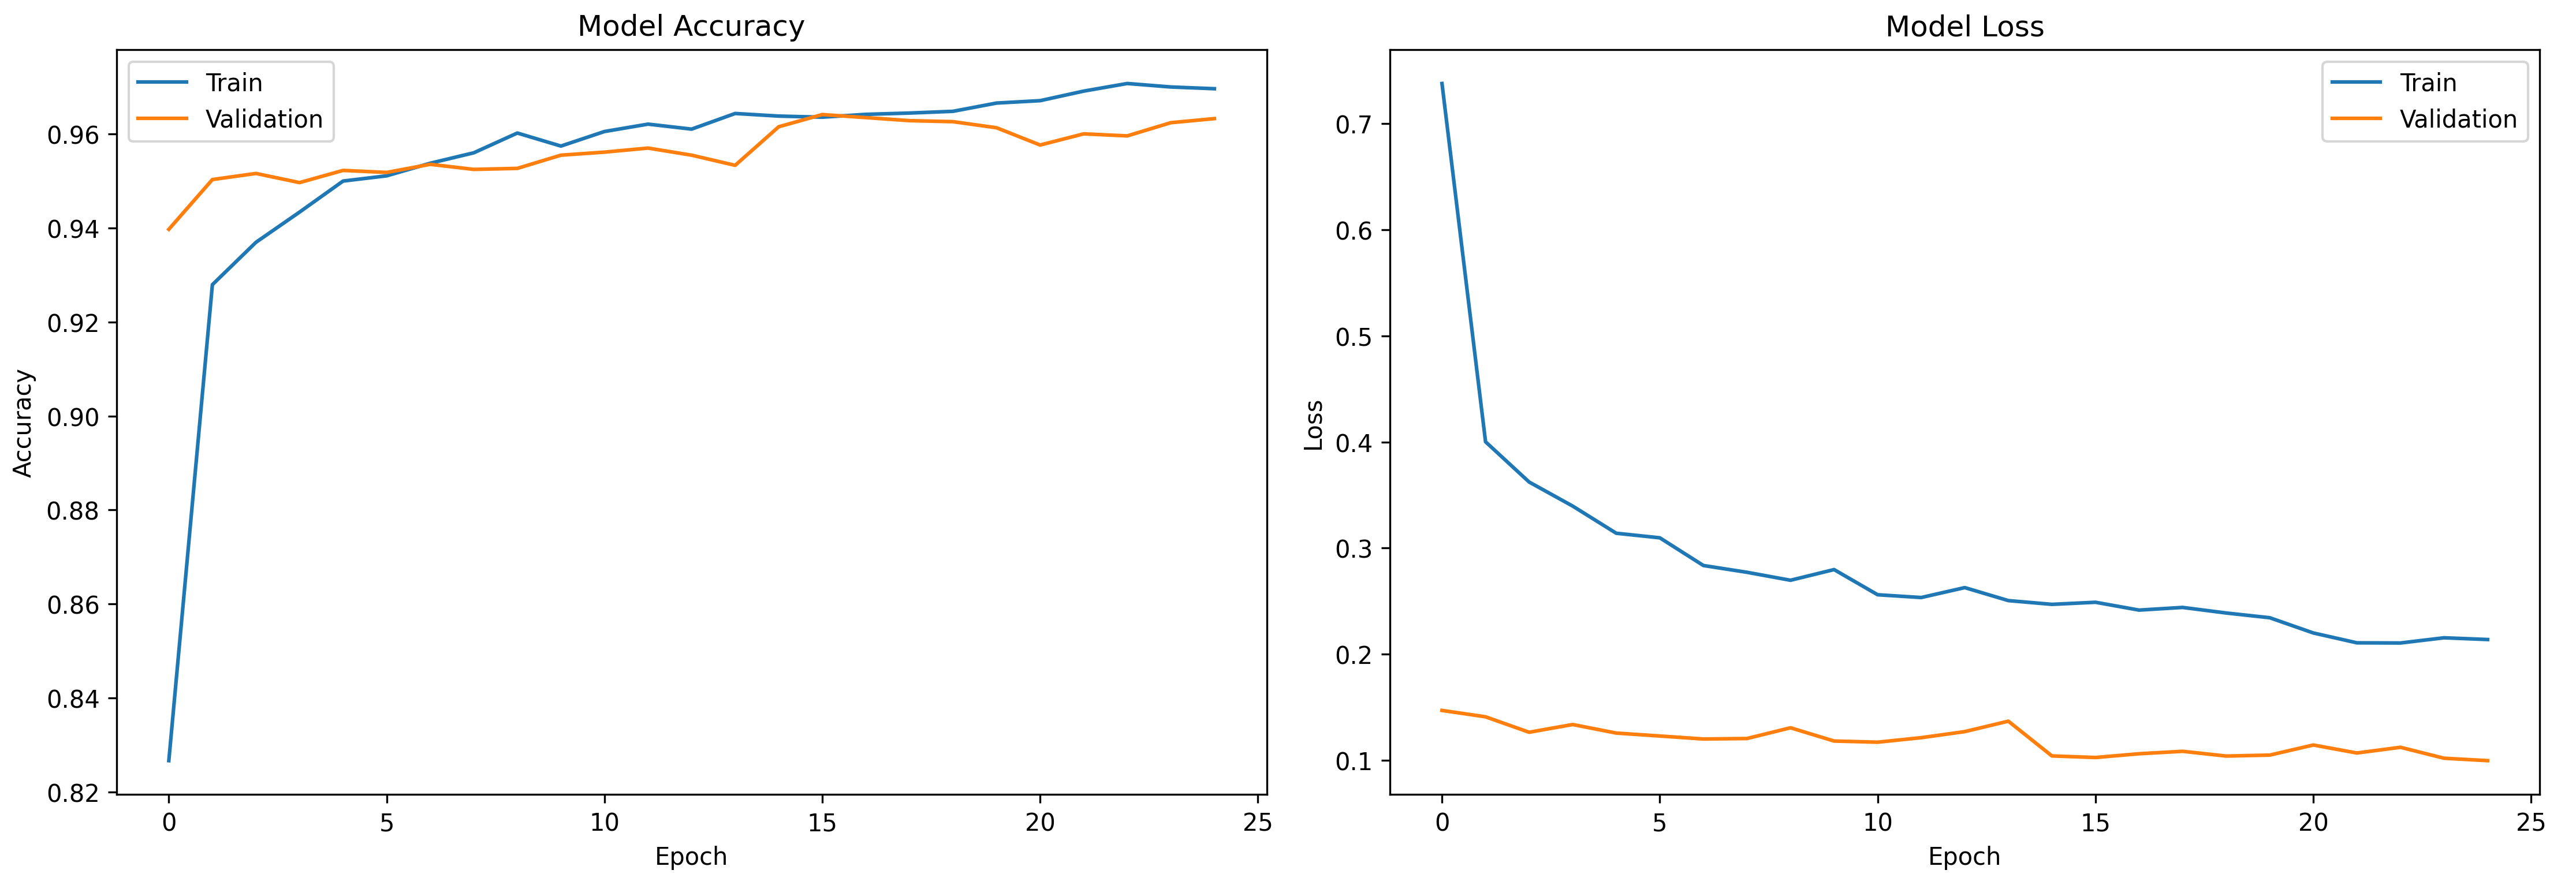
\includegraphics[width=0.9\textwidth]{figures/ConvNeXtLarge_training_history.png}
\caption{Training and validation accuracy (left) and loss (right) for ConvNeXtLarge, a top-group model, over the training split.}
\label{fig:traincurves}
\end{figure}

\begin{figure}[!htbp]
\centering
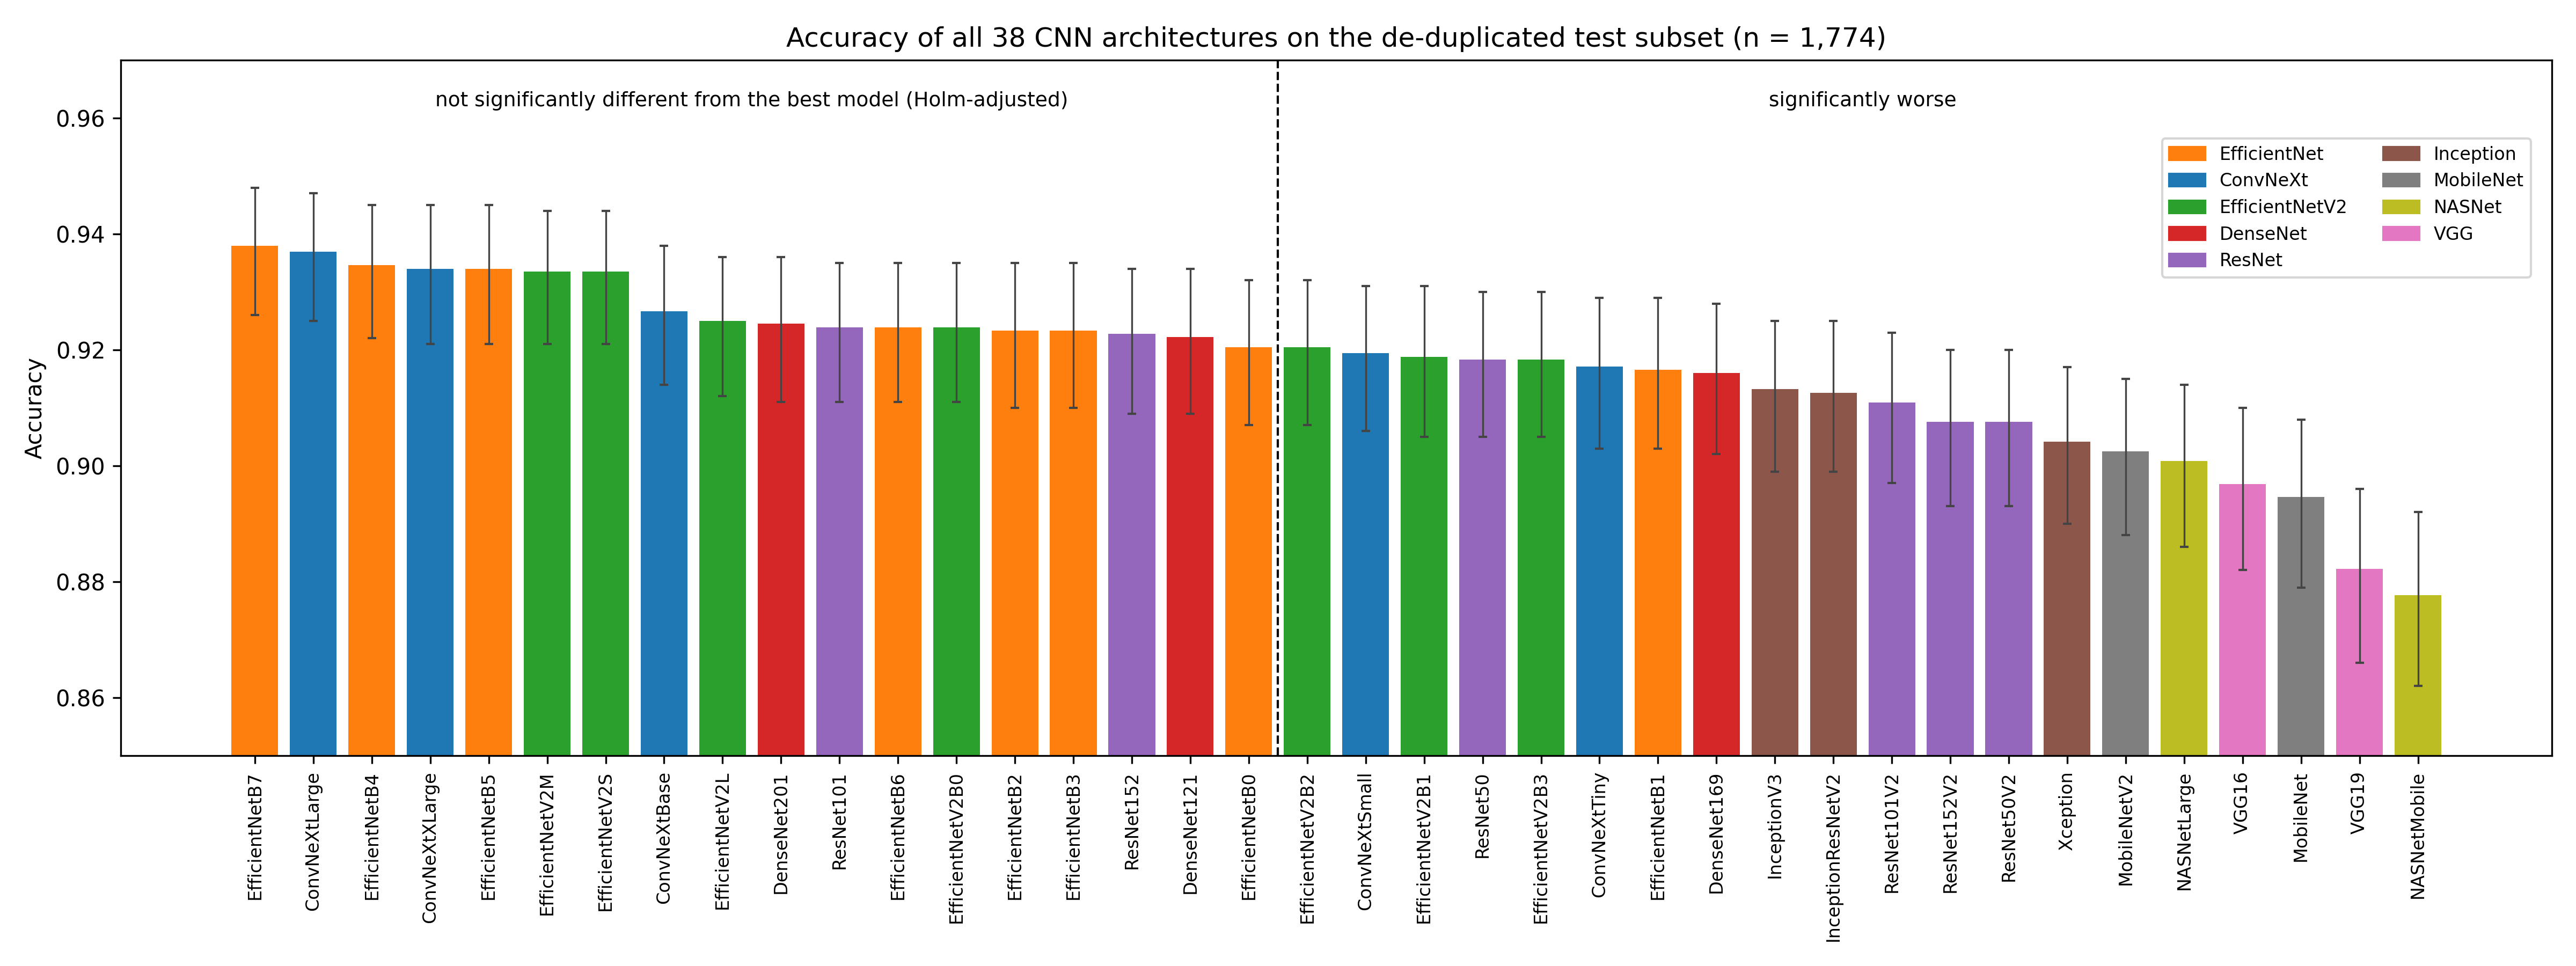
\includegraphics[width=1.0\textwidth]{figures/all_models_accuracy.png}
\caption{Accuracy of all 38 CNN architectures on the de-duplicated test subset ($n=1{,}774$), sorted in descending order and colour-coded by model family. Error bars show Wilson 95\% intervals. The first 18 models are not significantly different from the best model (Holm-adjusted McNemar's test).}
\label{fig:barchart}
\end{figure}

\subsubsection{Full 38-Model Benchmark.}
Table~\ref{tab:full38} reports results for all 38 architectures on the de-duplicated test subset, with Wilson 95\% intervals on accuracy and McNemar's test $p$-values against the best model on this subset. ROC-AUC and calibration for the seven top-group models are reported in Section~\ref{sec:calibration}. Accuracy ranges from 87.77\% (NASNetMobile) to 93.80\% (EfficientNetB7). Every model scores lower than on the original, non-de-duplicated test set, by 1.5 to 4.2 points (mean 2.5). This reflects both the removal of leaked images and the change in class mix: de-duplication removed mostly corn and potato images, which are classified almost perfectly, so the subset is dominated by the harder rice and wheat classes. The change should therefore not be read as the effect of leakage alone.

\begin{table}[p]
\centering
\caption{Full 38-model benchmark on the de-duplicated test subset ($n=1{,}774$; all 15 output classes). Acc: accuracy; subscript m: macro-averaged, w: weighted; MCC: Matthews correlation coefficient; CI: Wilson 95\% interval on accuracy; $p$ / $p_{\mathrm{Holm}}$: McNemar's test against EfficientNetB7 (best on this subset, selected post hoc), unadjusted / Holm-adjusted over 37 comparisons. Models above the rule (ranks 1 to 18) are not significantly different from the best model after Holm adjustment; those below it (ranks 19 to 38) are significantly worse. Bold: best per metric. ROC-AUC and calibration for the seven top-group models are given in Table~\ref{tab:calibration}.}
\label{tab:full38}
\scriptsize
\setlength{\tabcolsep}{2.5pt}
\resizebox{\textwidth}{!}{%
\begin{tabular}{rlccccccccrr}
\toprule
Rank & Model & Acc & 95\% CI & Prec$_m$ & Rec$_m$ & F1$_m$ & F1$_w$ & MCC & $p$ & $p_{\mathrm{Holm}}$ \\
\midrule
1 & EfficientNetB7 & \textbf{0.9380} & [0.926, 0.948] & \textbf{0.9248} & \textbf{0.9242} & \textbf{0.9229} & \textbf{0.9390} & \textbf{0.9322} & n/a & n/a \\
2 & ConvNeXtLarge & 0.9369 & [0.925, 0.947] & 0.9193 & 0.9222 & 0.9200 & 0.9375 & 0.9308 & 0.916 & 1.000 \\
3 & EfficientNetB4 & 0.9346 & [0.922, 0.945] & 0.9200 & 0.9204 & 0.9182 & 0.9348 & 0.9285 & 0.594 & 1.000 \\
4 & ConvNeXtXLarge & 0.9340 & [0.921, 0.945] & 0.9181 & 0.9193 & 0.9171 & 0.9343 & 0.9278 & 0.538 & 1.000 \\
5 & EfficientNetB5 & 0.9340 & [0.921, 0.945] & 0.9208 & 0.9188 & 0.9190 & 0.9348 & 0.9277 & 0.482 & 1.000 \\
6 & EfficientNetV2M & 0.9335 & [0.921, 0.944] & 0.8964 & 0.9197 & 0.9045 & 0.9344 & 0.9273 & 0.461 & 1.000 \\
7 & EfficientNetV2S & 0.9335 & [0.921, 0.944] & 0.9171 & 0.9205 & 0.9161 & 0.9333 & 0.9274 & 0.479 & 1.000 \\
8 & ConvNeXtBase & 0.9267 & [0.914, 0.938] & 0.9073 & 0.9084 & 0.9067 & 0.9268 & 0.9197 & 0.057 & 0.402 \\
9 & EfficientNetV2L & 0.9250 & [0.912, 0.936] & 0.8858 & 0.9063 & 0.8918 & 0.9246 & 0.9180 & 0.025 & 0.208 \\
10 & DenseNet201 & 0.9245 & [0.911, 0.936] & 0.8845 & 0.9088 & 0.8933 & 0.9257 & 0.9173 & 0.019 & 0.208 \\
11 & ResNet101 & 0.9239 & [0.911, 0.935] & 0.8835 & 0.9033 & 0.8901 & 0.9253 & 0.9167 & 0.020 & 0.208 \\
12 & EfficientNetB6 & 0.9239 & [0.911, 0.935] & 0.8822 & 0.9074 & 0.8842 & 0.9251 & 0.9172 & 0.007 & 0.111 \\
13 & EfficientNetV2B0 & 0.9239 & [0.911, 0.935] & 0.9058 & 0.9016 & 0.9032 & 0.9245 & 0.9165 & 0.019 & 0.208 \\
14 & EfficientNetB2 & 0.9233 & [0.910, 0.935] & 0.9052 & 0.9092 & 0.9057 & 0.9248 & 0.9162 & 0.017 & 0.206 \\
15 & EfficientNetB3 & 0.9233 & [0.910, 0.935] & 0.9083 & 0.9075 & 0.9057 & 0.9252 & 0.9163 & 0.012 & 0.162 \\
16 & ResNet152 & 0.9228 & [0.909, 0.934] & 0.8824 & 0.9044 & 0.8896 & 0.9246 & 0.9156 & 0.011 & 0.156 \\
17 & DenseNet121 & 0.9222 & [0.909, 0.934] & 0.8831 & 0.9075 & 0.8914 & 0.9238 & 0.9150 & 0.009 & 0.141 \\
18 & EfficientNetB0 & 0.9205 & [0.907, 0.932] & 0.8799 & 0.8959 & 0.8853 & 0.9204 & 0.9128 & 0.005 & 0.081 \\
\midrule
19 & EfficientNetV2B2 & 0.9205 & [0.907, 0.932] & 0.8821 & 0.9007 & 0.8862 & 0.9213 & 0.9132 & 0.002 & 0.042 \\
20 & ConvNeXtSmall & 0.9194 & [0.906, 0.931] & 0.8809 & 0.9008 & 0.8863 & 0.9217 & 0.9120 & 0.002 & 0.029 \\
21 & EfficientNetV2B1 & 0.9188 & [0.905, 0.931] & 0.8765 & 0.8951 & 0.8824 & 0.9193 & 0.9111 & 0.002 & 0.035 \\
22 & ResNet50 & 0.9183 & [0.905, 0.930] & 0.9034 & 0.9041 & 0.9002 & 0.9204 & 0.9110 & 0.001 & 0.029 \\
23 & EfficientNetV2B3 & 0.9183 & [0.905, 0.930] & 0.9007 & 0.9012 & 0.8999 & 0.9199 & 0.9105 & $<$0.001 & 0.016 \\
24 & ConvNeXtTiny & 0.9171 & [0.903, 0.929] & 0.8781 & 0.9018 & 0.8846 & 0.9184 & 0.9096 & $<$0.001 & 0.016 \\
25 & EfficientNetB1 & 0.9166 & [0.903, 0.929] & 0.9004 & 0.8951 & 0.8945 & 0.9172 & 0.9089 & $<$0.001 & 0.009 \\
26 & DenseNet169 & 0.9160 & [0.902, 0.928] & 0.8995 & 0.8990 & 0.8972 & 0.9174 & 0.9082 & $<$0.001 & 0.005 \\
27 & InceptionV3 & 0.9132 & [0.899, 0.925] & 0.8610 & 0.8909 & 0.8699 & 0.9139 & 0.9048 & $<$0.001 & 0.001 \\
28 & InceptionResNetV2 & 0.9126 & [0.899, 0.925] & 0.8760 & 0.8918 & 0.8807 & 0.9136 & 0.9042 & $<$0.001 & 0.002 \\
29 & ResNet101V2 & 0.9109 & [0.897, 0.923] & 0.8940 & 0.8946 & 0.8929 & 0.9123 & 0.9025 & $<$0.001 & 0.001 \\
30 & ResNet152V2 & 0.9076 & [0.893, 0.920] & 0.8719 & 0.8888 & 0.8746 & 0.9088 & 0.8992 & $<$0.001 & $<$0.001 \\
31 & ResNet50V2 & 0.9076 & [0.893, 0.920] & 0.8921 & 0.8936 & 0.8905 & 0.9090 & 0.8990 & $<$0.001 & $<$0.001 \\
32 & Xception & 0.9042 & [0.890, 0.917] & 0.8711 & 0.8882 & 0.8741 & 0.9055 & 0.8954 & $<$0.001 & $<$0.001 \\
33 & MobileNetV2 & 0.9025 & [0.888, 0.915] & 0.8669 & 0.8833 & 0.8706 & 0.9036 & 0.8934 & $<$0.001 & $<$0.001 \\
34 & NASNetLarge & 0.9008 & [0.886, 0.914] & 0.8910 & 0.8832 & 0.8843 & 0.9018 & 0.8915 & $<$0.001 & $<$0.001 \\
35 & VGG16 & 0.8968 & [0.882, 0.910] & 0.8835 & 0.8802 & 0.8783 & 0.8995 & 0.8875 & $<$0.001 & $<$0.001 \\
36 & MobileNet & 0.8946 & [0.879, 0.908] & 0.8700 & 0.8687 & 0.8527 & 0.8919 & 0.8858 & $<$0.001 & $<$0.001 \\
37 & VGG19 & 0.8822 & [0.866, 0.896] & 0.8696 & 0.8636 & 0.8592 & 0.8825 & 0.8719 & $<$0.001 & $<$0.001 \\
38 & NASNetMobile & 0.8777 & [0.862, 0.892] & 0.8329 & 0.8438 & 0.8330 & 0.8765 & 0.8660 & $<$0.001 & $<$0.001 \\
\bottomrule
\end{tabular}}
\end{table}

\subsubsection{Architecture Family Analysis.}
Five of the seven top-group models are EfficientNet or EfficientNetV2 variants (B7, B4, B5, V2M, V2S), and the other two are ConvNeXt (Large and XLarge); no family is clearly ahead on this subset. Within ConvNeXt, accuracy rises with size from Tiny (91.71\%) to Large (93.69\%), and XLarge (93.40\%) is no better than Large; Small and Tiny are significantly worse than the best model after Holm adjustment ($p_{\mathrm{Holm}}=0.029$ and $0.016$), while Base (92.67\%) is not ($p_{\mathrm{Holm}}=0.40$). EfficientNetV2S offers the best accuracy/latency compromise inside the top group (93.35\% at 9.7\,ms per image, batched). MobileNet and MobileNetV2 remain the lightest options for real-time on-device inference but are 4.3 and 3.6 points below the best model, a statistically significant gap; VGG, MobileNet and NASNet variants are the weakest (87.8 to 90.3\%).

\subsubsection{Statistical Significance.}
\label{sec:stat_sig}
Each model's per-image correctness on the de-duplicated test subset was compared with that of the best model on this subset (EfficientNetB7) using McNemar's test (an exact binomial test when fewer than 25 discordant pairs, a continuity-corrected $\chi^2$ test otherwise), which is appropriate because all models are scored on identical images. Because 37 comparisons are made, Holm-adjusted $p$-values are reported alongside unadjusted ones; Wilson 95\% intervals are given for each accuracy.

Seventeen of the 37 other models, including the other six models of the top seven and ConvNeXtBase, are not significantly different from EfficientNetB7 after Holm adjustment. Twenty, from EfficientNetV2B2 (92.05\%, $p_{\mathrm{Holm}}=0.042$) downward, are significantly worse. Without adjustment the boundary would lie higher, at EfficientNetV2L (92.50\%, $p=0.025$). The accuracy intervals are about $\pm1.1$ percentage points wide, so differences of less than roughly 1.5 to 2 points between individual models cannot be resolved with $n=1{,}774$. The ranking among the top models is unstable: EfficientNetB7 ranks first in 40\% of 2{,}000 bootstrap resamples of the test images and ConvNeXtLarge in 24\%, and the top seven together account for over 99\% of first places. Three further caveats apply. The reference model was selected on the same test images, which favours it. Each model was trained once, so training variance is not captured. And ``not significantly different'' is not evidence of equivalence.
\subsubsection{Discrimination and Calibration.}
\label{sec:calibration}
For the seven models in the top group, we also computed one-vs-rest ROC-AUC and the expected calibration error (ECE, 10 equal-width confidence bins) on the de-duplicated test subset (Table~\ref{tab:calibration}). Macro ROC-AUC lies between 0.9963 and 0.9966 for all seven models, so they separate the classes almost equally well and AUC does not distinguish them. Calibration differs more. ECE ranges from 0.0158 (EfficientNetV2M) to 0.0325 (ConvNeXtXLarge), and every model is somewhat over-confident: mean confidence exceeds accuracy by 1.6 to 3.3 points, most for the two ConvNeXt models. The deployed EfficientNetV2S has an ECE of 0.0228, with a mean confidence of 95.4\% against an accuracy of 93.4\%; its reliability diagram and per-class ROC curves are shown in Figure~\ref{fig:calibration}. Per-class AUC values for Potato Healthy ($n=2$) and Potato Early Blight ($n=22$) rest on too few positive examples to be interpreted.

\begin{table}[!htbp]
\centering
\caption{Discrimination and calibration of the seven top-group models on the de-duplicated test subset ($n = 1{,}774$). Macro ROC-AUC is one-vs-rest, averaged over classes; ECE uses 10 equal-width confidence bins. Gap = mean confidence minus accuracy.}
\label{tab:calibration}
\small
\begin{tabular}{lccccc}
\toprule
Model & Accuracy & Macro AUC & ECE & Mean conf. & Gap (pts) \\
\midrule
EfficientNetB7  & 0.9380 & 0.9965 & 0.0235 & 0.9553 & 1.7 \\
ConvNeXtLarge   & 0.9369 & 0.9965 & 0.0277 & 0.9646 & 2.8 \\
EfficientNetB4  & 0.9346 & 0.9963 & 0.0250 & 0.9592 & 2.5 \\
ConvNeXtXLarge  & 0.9340 & 0.9963 & 0.0325 & 0.9665 & 3.3 \\
EfficientNetB5  & 0.9340 & 0.9966 & 0.0199 & 0.9525 & 1.9 \\
EfficientNetV2M & 0.9335 & 0.9965 & 0.0158 & 0.9493 & 1.6 \\
EfficientNetV2S & 0.9335 & 0.9964 & 0.0228 & 0.9538 & 2.0 \\
\bottomrule
\end{tabular}
\end{table}

\begin{figure}[!htbp]
\centering
\begin{subfigure}[b]{0.48\textwidth}
  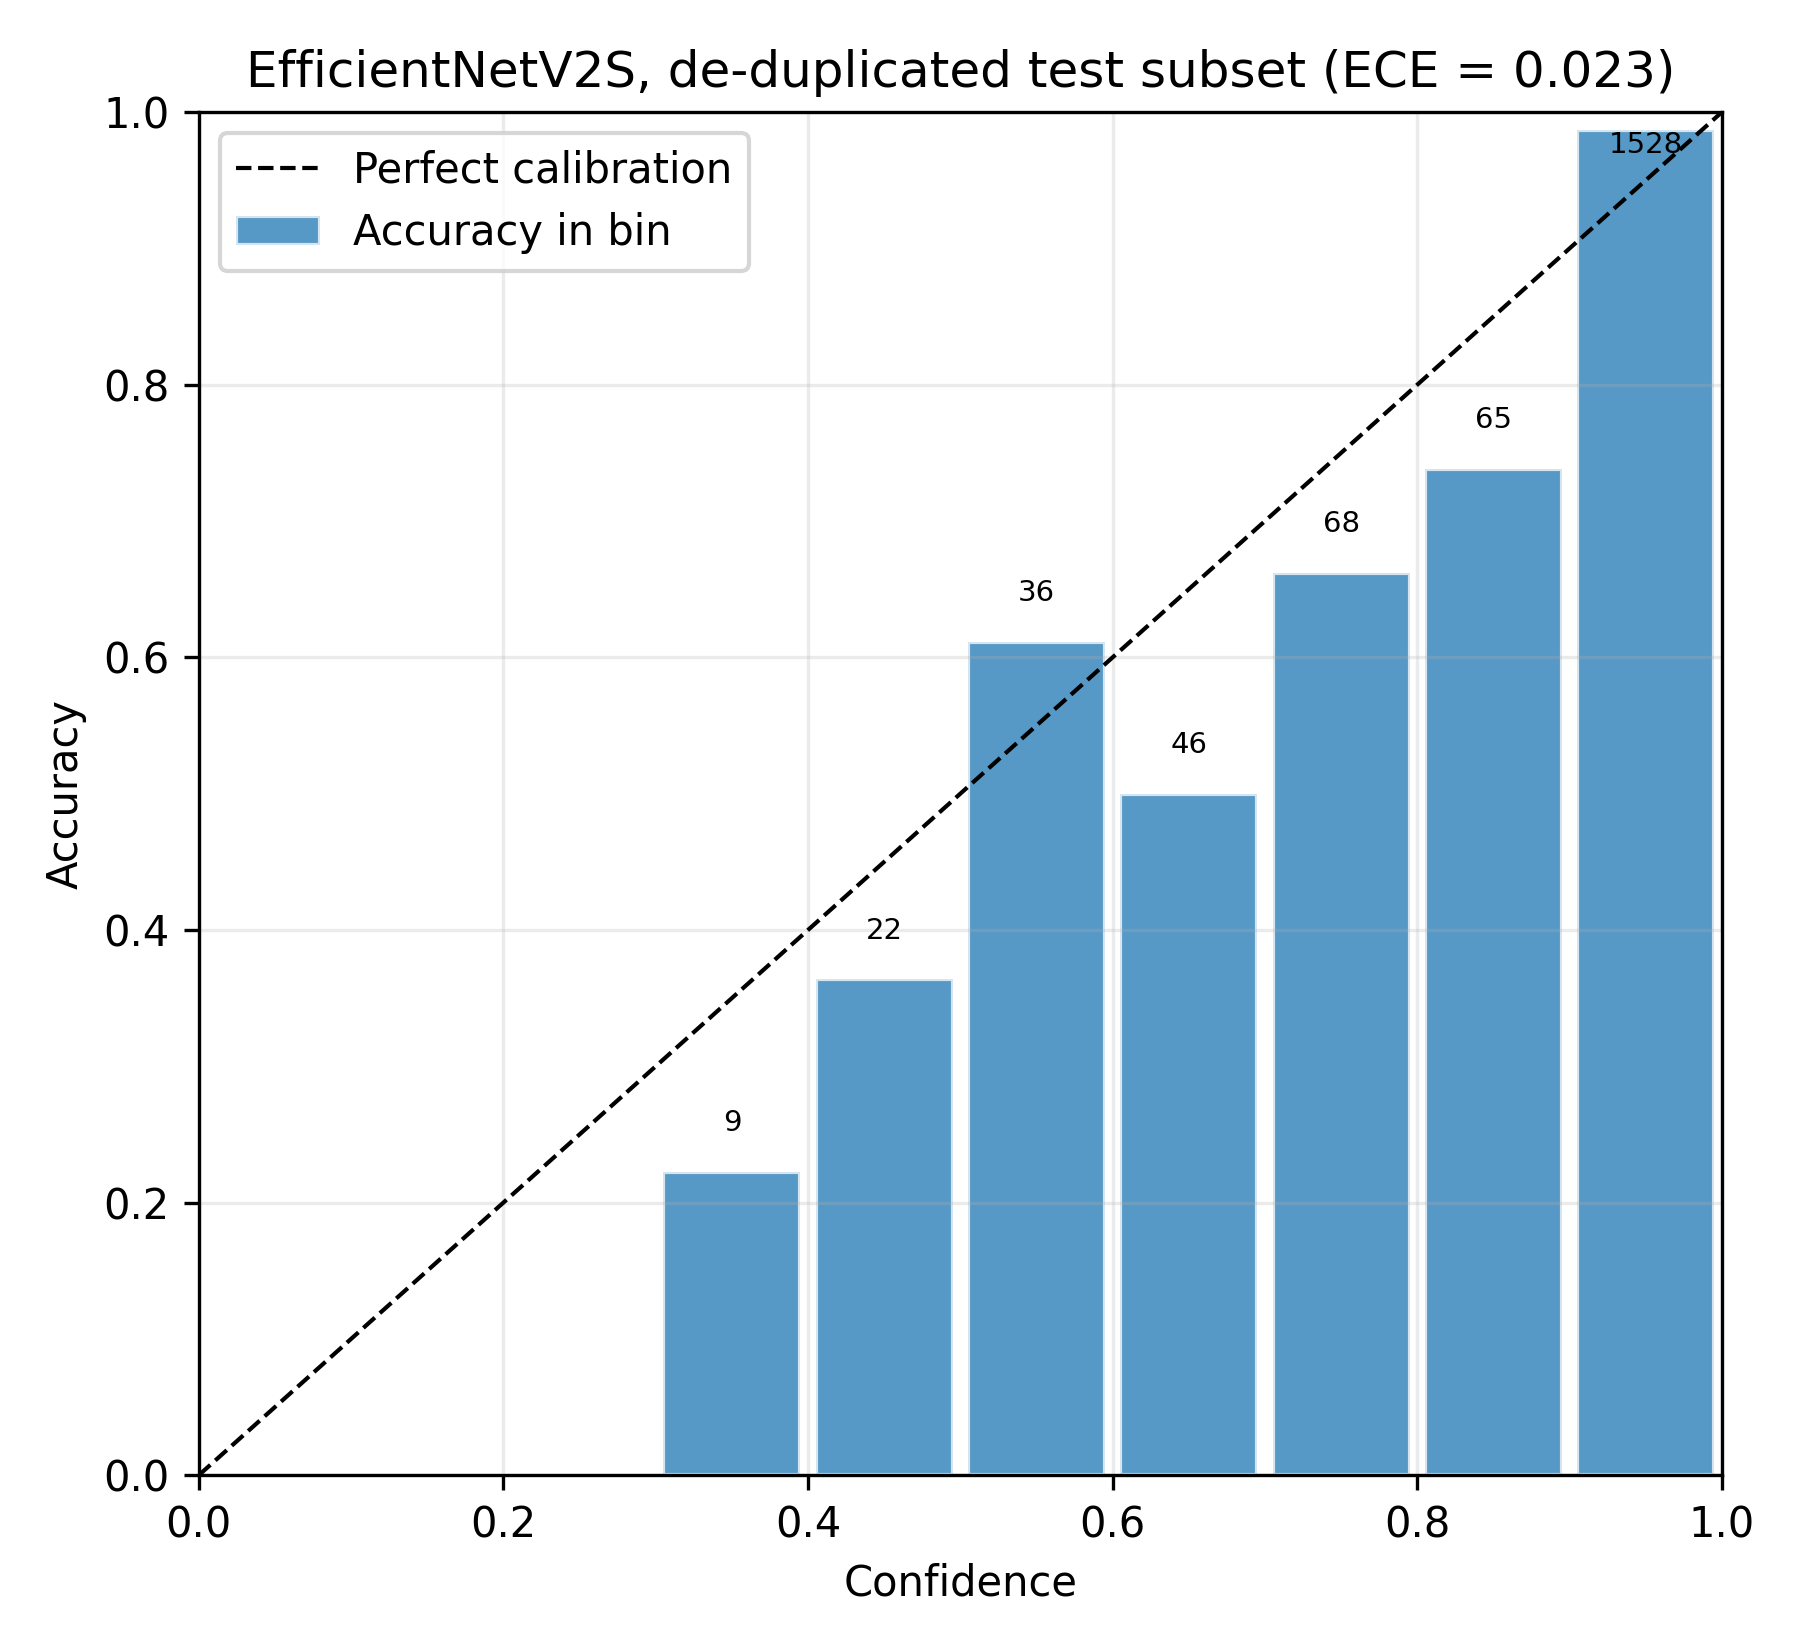
\includegraphics[width=\textwidth]{figures/reliability_EfficientNetV2S.png}
  \caption{Reliability diagram}
\end{subfigure}
\hfill
\begin{subfigure}[b]{0.48\textwidth}
  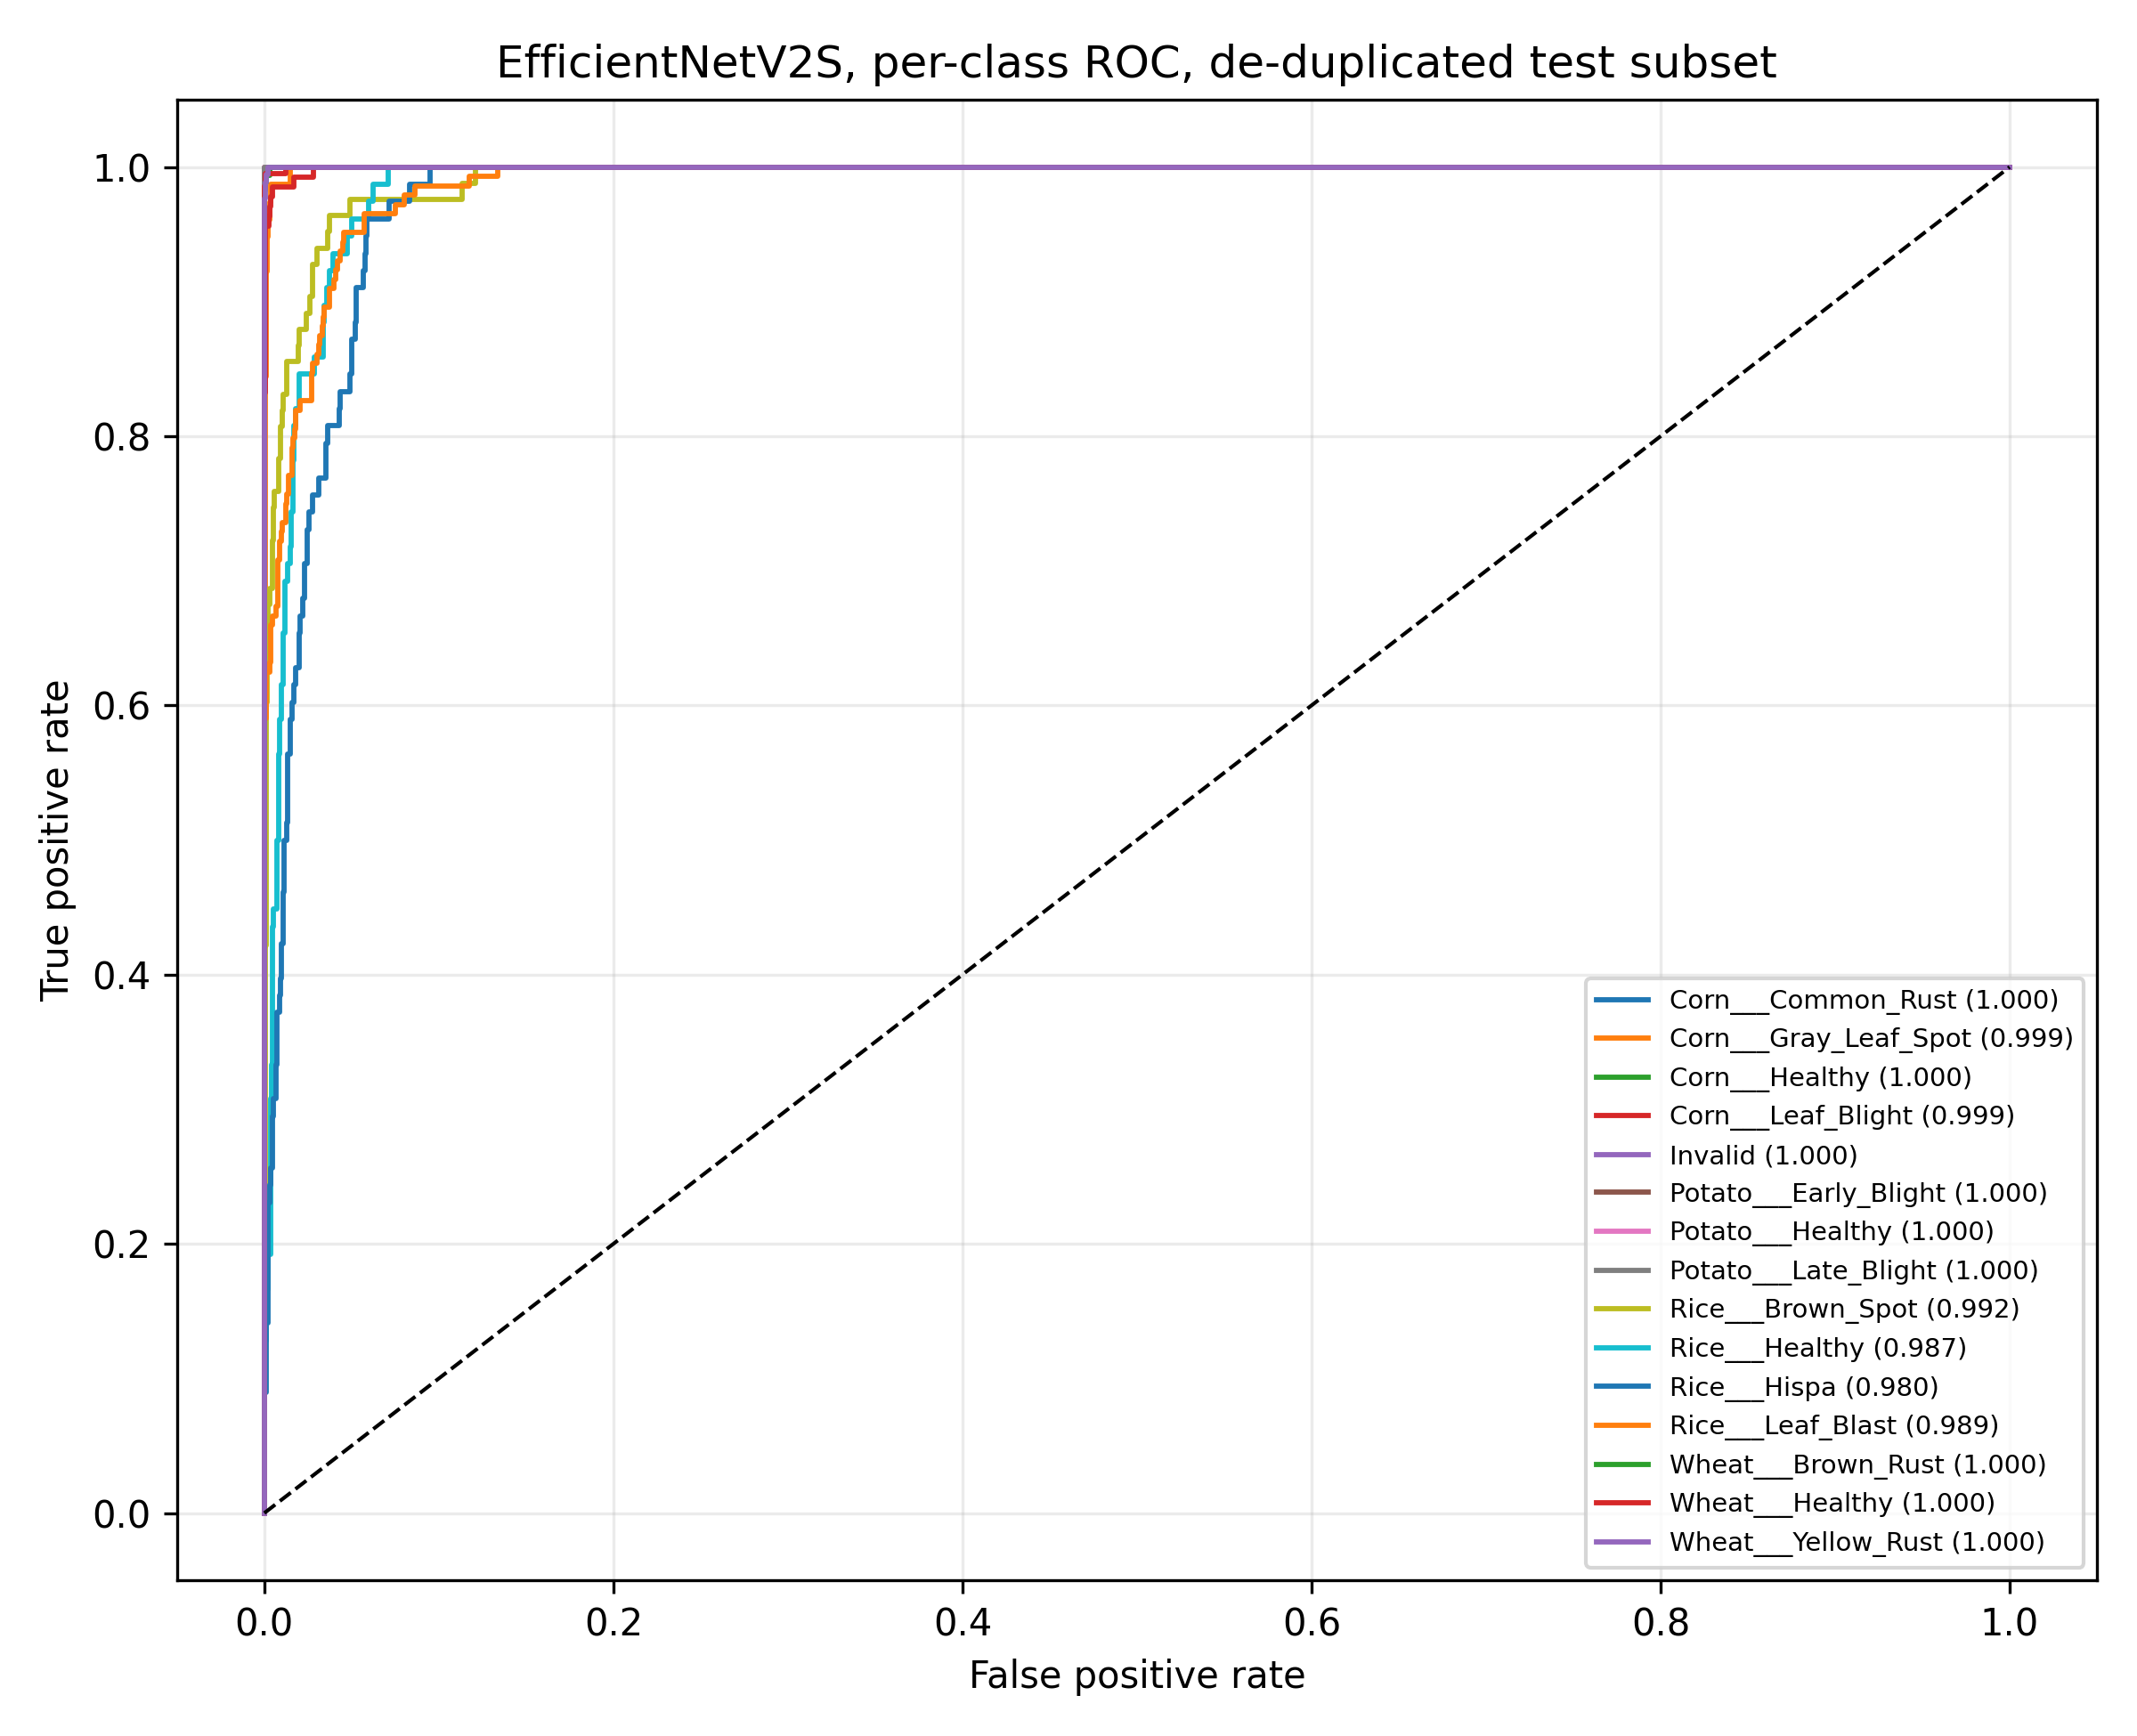
\includegraphics[width=\textwidth]{figures/roc_EfficientNetV2S.png}
  \caption{Per-class ROC curves}
\end{subfigure}
\caption{Reliability diagram (a) and per-class ROC curves (b) for EfficientNetV2S on the de-duplicated test subset ($n = 1{,}774$). Bars above the diagonal would indicate under-confidence; bars below it, over-confidence.}
\label{fig:calibration}
\end{figure}

\subsubsection{Accuracy-Efficiency Trade-off.}
Figure~\ref{fig:accvsspeed} plots de-duplicated test accuracy against batched per-image inference time (Section~\ref{sec:metrics}) for all 38 models. Within the top group, EfficientNetV2S is fastest (9.7\,ms), followed by EfficientNetB4 (10.6\,ms), EfficientNetV2M (15.1\,ms), EfficientNetB5 (15.7\,ms), ConvNeXtLarge (17.9\,ms), ConvNeXtXLarge (28.0\,ms) and EfficientNetB7 (34.1\,ms). EfficientNetB3 (8.0\,ms) is slightly faster than EfficientNetV2S but about one point less accurate (92.33\% versus 93.35\%), a difference that is not significant against the best model after adjustment ($p_{\mathrm{Holm}}=0.16$). Legacy architectures (VGG, NASNetMobile) cluster in the lower-left quadrant, offering neither competitive accuracy nor speed. These times are batched throughput measurements, not single-image latency.

\begin{figure}[!htbp]
\centering
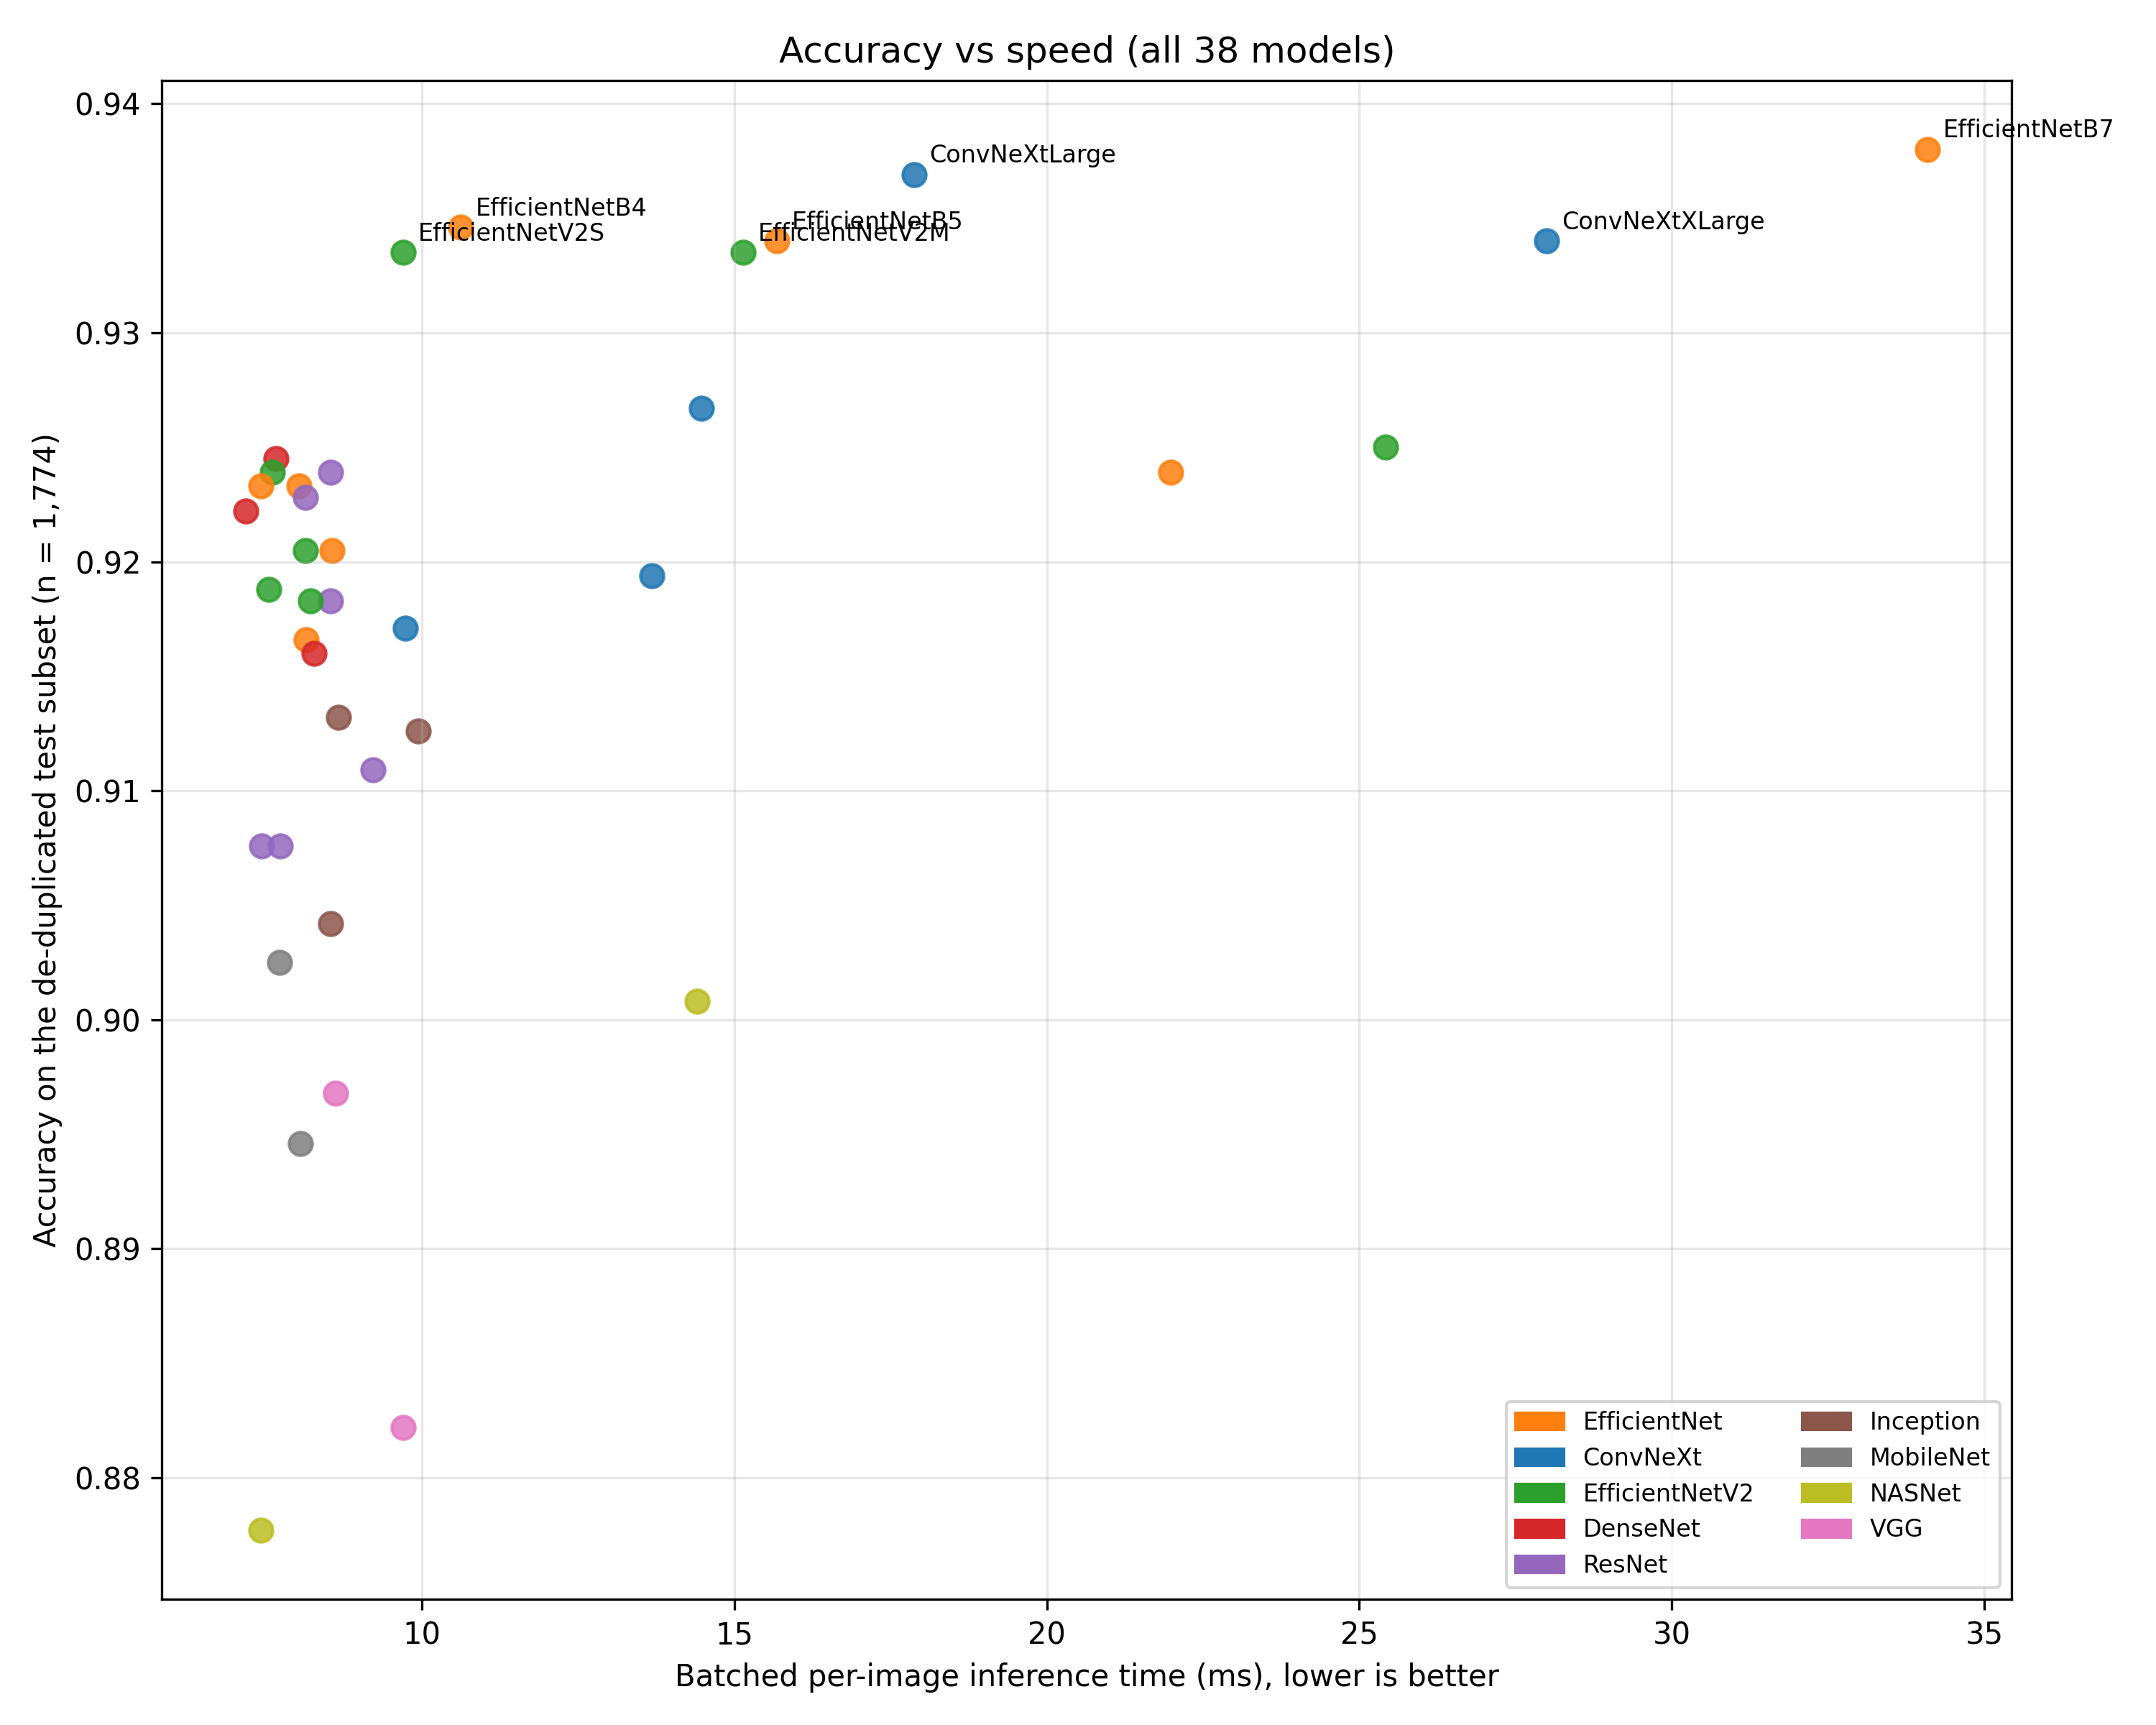
\includegraphics[width=0.8\textwidth]{figures/accuracy_vs_speed.png}
\caption{Accuracy on the de-duplicated test subset versus batched per-image inference time for all 38 models, colour-coded by model family.}
\label{fig:accvsspeed}
\end{figure}

\subsubsection{Comparison with Prior Work.}
Table~\ref{tab:priorwork} situates our results within the existing literature. Our best Stage 1 accuracies on the de-duplicated subset (93.80\% for EfficientNetB7 and 93.69\% for ConvNeXtLarge) are 5.5 to 5.8 points below the figures reported by Mohanty et al.~\cite{mohanty2016} (99.35\%) and Ferentinos~\cite{ferentinos2018} (99.5\%). The comparison is indicative only: those studies use PlantVillage images captured under controlled conditions, and test sets, class sets and splits differ. De-duplication here removed most corn and potato images, leaving a subset dominated by the rice and wheat classes on which our errors concentrate (Section~\ref{sec:perclass}), and the corn and potato classes appear to contain PlantVillage-derived images (Section~\ref{sec:plantvillage}).
Our Stage~2 mAP@0.5 of 49.3\% was obtained with a severity-aware model trained on 2,256 
automatically annotated images and evaluated on a hash-audited held-out split 
(Section~\ref{sec:detection}). The manual-only baseline (35\% mAP@0.5) used fewer images, 
different labels and a different setup, and was not re-run on this split, so the two figures 
cannot be compared directly.

\begin{table}[!htbp]
\centering
\caption{Comparison with related work.}
\label{tab:priorwork}
\setlength{\tabcolsep}{4pt}
{\small
\begin{tabular}{L{3.0cm}L{2.5cm}L{2.5cm}ll}
\toprule
\textbf{Study} & \textbf{Dataset} & \textbf{Model} &
\textbf{Metric} & \textbf{Result}\\
\midrule
Mohanty et al.~\cite{mohanty2016} & PlantVillage & GoogLeNet & Accuracy & 99.35\%\\
Geetharamani \& Pandian~\cite{geetharamani2019} & PlantVillage & 9-layer CNN & Accuracy & 96.46\%\\
Ferentinos~\cite{ferentinos2018} & PlantVillage & AlexNet/VGG & Accuracy & 99.5\%\\
Nawaz et al.~\cite{nawaz2023} & PlantVillage & VGG-19 Faster RCNN & mAP & 0.87\\
Nawaz et al.~\cite{nawaz2023} & PlantVillage & VGG-19 Faster RCNN & Accuracy & 99.51\%\\
Kadry et al.~\cite{kadry2025} & Insect DB & Fused EfficientNet & Accuracy & 98.3\%\\
Das et al.~\cite{das2024} (survey) & Multiple & ResNet/EfficientNet & Accuracy & 85 to 98\%\\
\midrule
\textbf{Ours (Stage 1)} & Bangladeshi (de-duplicated subset) & EfficientNetB7 / ConvNeXtLarge & Accuracy & \textbf{93.80\% / 93.69\%}\\
\textbf{Ours (Stage 2)} & Bangladeshi & Severity-aware RCNN & mAP@0.5 & \textbf{0.493}\\
\bottomrule
\end{tabular}
}
\end{table}

\subsubsection{Per-Class Analysis and Error Analysis.}
\label{sec:perclass}
Table~\ref{tab:perclass} reports per-class precision, recall and F1 for ConvNeXtLarge on the 14 disease and healthy classes of the de-duplicated test subset (1,541 of its 1,774 images; Invalid, $n=233$, is excluded from this table and its macro average, whereas headline accuracy covers all 15 output classes). Because de-duplication removed most corn and potato images, class support varies widely, and two potato classes with fewer than 30 images (Early Blight, $n=22$; Healthy, $n=2$) are marked and should not be interpreted. Ten of the 14 classes reach F$_1\ge0.87$ (eight of the 12 classes with at least 30 images). The four lowest are all rice classes: Rice Hispa (0.636), Rice Healthy (0.686), Rice Leaf Blast (0.812) and Rice Brown Spot (0.831), followed by Corn Gray Leaf Spot (0.897). All 78 Rice Hispa and all 78 Rice Healthy test images were retained by de-duplication, so their recall values and the confusion counts below are unchanged from the original test set (their precision depends on the other retained classes). The dominant confusion is the Rice Hispa / Rice Healthy pair, and it is bidirectional: 19 of 78 Rice Hispa test images (24.4\%) are misclassified as Rice Healthy, and 13 of 78 Rice Healthy images (16.7\%) as Rice Hispa.

\begin{table}[!htbp]
\centering
\caption{Per-class performance of ConvNeXtLarge on the de-duplicated test subset (14 disease and healthy classes; the Invalid class, $n=233$, is excluded). Support is the number of test images. $^\dagger$Fewer than 30 images; not interpretable. The macro average is over the 14 classes shown; over the 12 classes with at least 30 images it is 0.899 / 0.903 / 0.900.}
\label{tab:perclass}
\small
\begin{tabular}{lcccc}
\toprule
Class & Precision & Recall & F1 & Support \\
\midrule
Corn Common Rust & 1.000 & 0.994 & 0.997 & 172 \\
Corn Gray Leaf Spot & 0.886 & 0.909 & 0.897 & 77 \\
Corn Healthy & 1.000 & 1.000 & 1.000 & 167 \\
Corn Leaf Blight & 0.949 & 0.942 & 0.945 & 137 \\
Potato Early Blight$^\dagger$ & 1.000 & 1.000 & 1.000 & 22 \\
Potato Healthy$^\dagger$ & 1.000 & 1.000 & 1.000 & 2 \\
Potato Late Blight & 1.000 & 1.000 & 1.000 & 30 \\
Rice Brown Spot & 0.831 & 0.831 & 0.831 & 83 \\
Rice Healthy & 0.619 & 0.769 & 0.686 & 78 \\
Rice Hispa & 0.645 & 0.628 & 0.636 & 78 \\
Rice Leaf Blast & 0.866 & 0.764 & 0.812 & 144 \\
Wheat Brown Rust & 0.994 & 1.000 & 0.997 & 169 \\
Wheat Healthy & 1.000 & 0.995 & 0.998 & 209 \\
Wheat Yellow Rust & 1.000 & 1.000 & 1.000 & 173 \\
\midrule
Macro avg (14 classes) & 0.914 & 0.917 & 0.914 & 1541 \\
\bottomrule
\end{tabular}
\end{table}

The confusion matrix (Figure~\ref{fig:confmat}) shows that the
dominant error pattern involves visually similar rice categories,
bidirectionally between Rice Hispa and Rice Healthy as described above. Both classes share a similar green texture with
minor surface irregularities, which likely drives the confusion in
both directions.

\begin{figure}[!htbp]
\centering
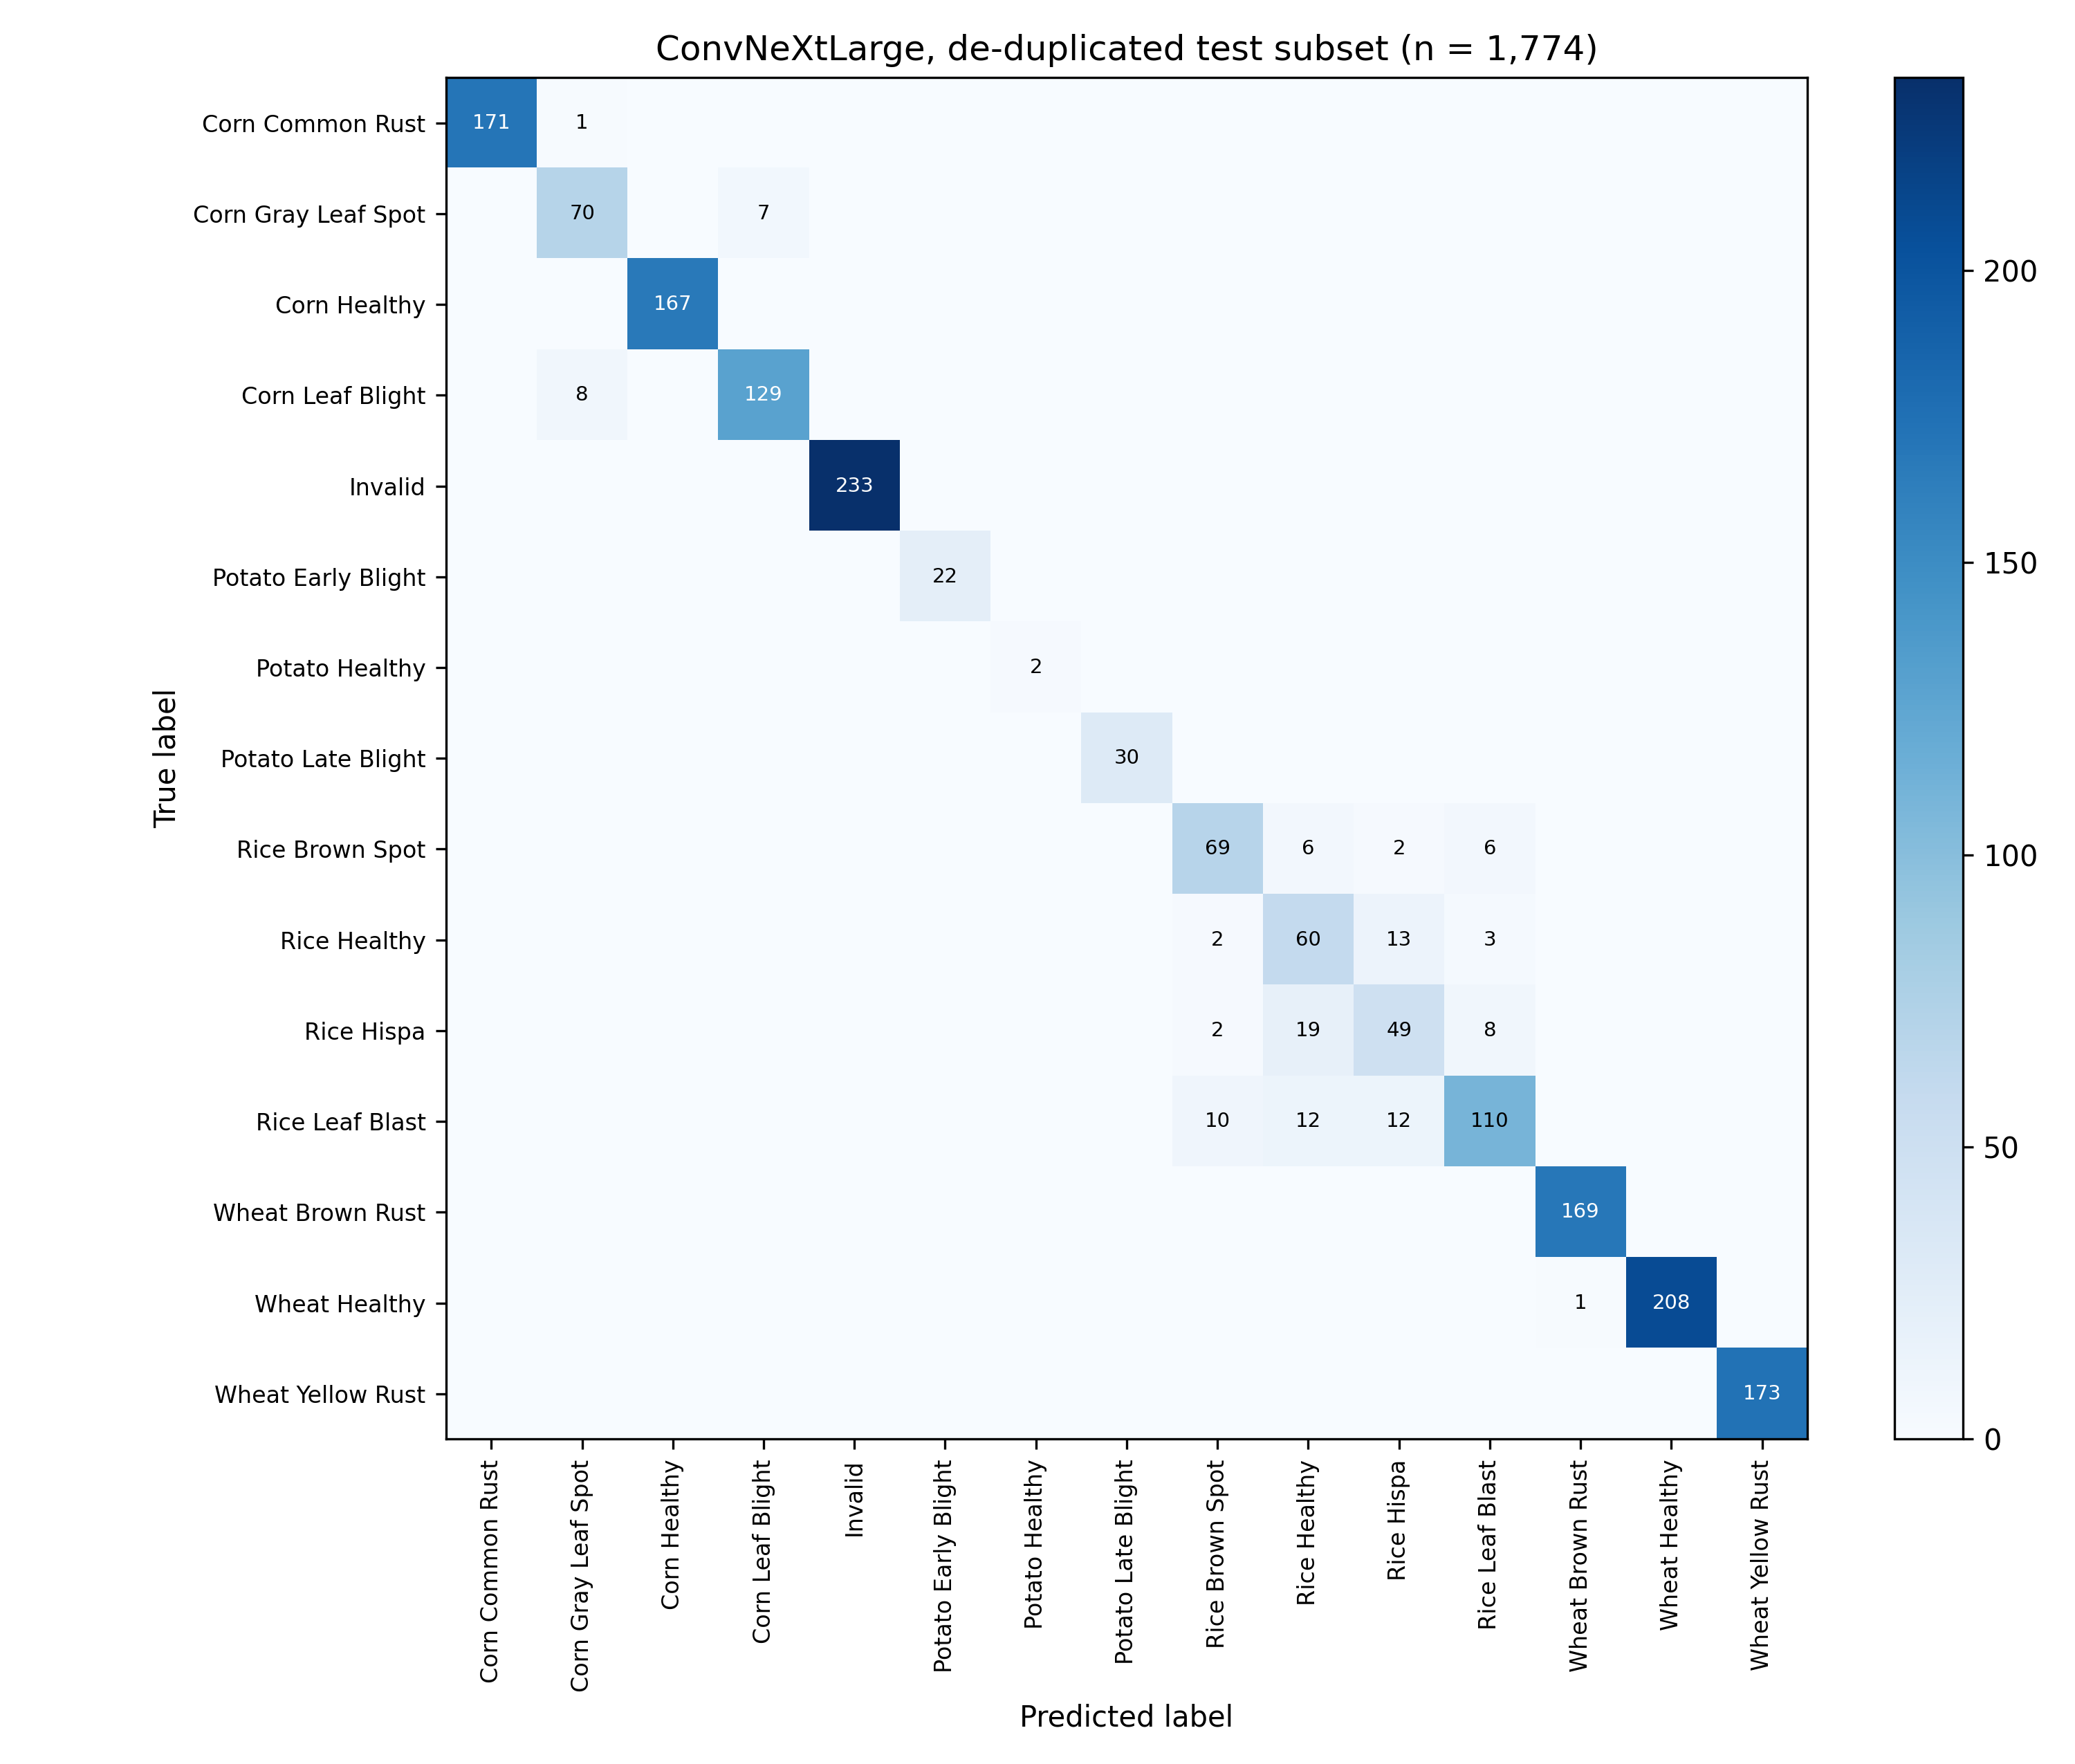
\includegraphics[width=0.9\textwidth]{figures/ConvNeXtLarge_confusion_matrix.png}
\caption{Confusion matrix for ConvNeXtLarge on the de-duplicated test subset ($n=1{,}774$). Errors concentrate in the rice classes, with a bidirectional Rice Hispa / Rice Healthy confusion.}
\label{fig:confmat}
\end{figure}

Full Grad-CAM heatmaps for these examples are presented in
Section~\ref{sec:gradcam_full} (Figure~\ref{fig:gradcam}).

\subsubsection*{Deployment Recommendations.}
For cloud servers, any of the seven top-group models is supported by the data, and the choice can be made on latency and memory (for example ConvNeXtLarge, 93.69\%, 17.9\,ms, or EfficientNetB7, 93.80\%, 34.1\,ms). For edge devices (drones, field gateways), EfficientNetV2S (93.35\%, 9.7\,ms, about 81.7\,MB) is the fastest model in the top group. For mobile sensors, MobileNetV2 (90.25\%, about 11.7\,MB) is the lightweight option when memory is the binding constraint, at a statistically significant accuracy cost of about 3.6 points relative to the best model.

\paragraph{Why EfficientNetV2S is the deployed classifier.} EfficientNetV2S was chosen as the deployed classifier during system integration, before the duplicate audit, and the audit did not change this choice. On the de-duplicated test subset its accuracy (93.35\%) is 0.45 points below the best model, EfficientNetB7 (93.80\%), and the difference is not significant after Holm adjustment. Among the seven models that cannot be separated from the best, it has the shortest batched inference time (9.7\,ms per image, against 10.6 to 34.1\,ms for the others) and, at 81.7\,MB, is among the smallest; only EfficientNetB4 (72.5\,MB) is smaller, and it is slower (10.6\,ms). Its calibration is in the middle of the top group (ECE 0.0228; Table~\ref{tab:calibration}). Since the dynamic severity pipeline is meant to run on modest hardware, we judged this speed worth a loss of under half a point.
\subsubsection{Discussion.}
Several patterns are worth drawing out. First, the benchmark does not single out one architecture: seven models from two families are statistically tied at 93.4 to 93.8\%, so the choice among them is better made on size and latency than on accuracy. Second, accuracy does not increase monotonically with ConvNeXt size: Large (93.69\%) is nominally above XLarge (93.40\%) and Base (92.67\%), but these differences are within the resolution of the test set, and since each model was trained once, and ConvNeXtLarge and ConvNeXtXLarge were trained with a frozen backbone for at most 25 epochs, unlike the EfficientNet models, we cannot separate under-training, over-parameterisation and run-to-run variance. Third, ConvNeXt's strong transfer is consistent with its design, which modernises a standard ResNet with large depthwise kernels, inverted bottlenecks and layer normalisation~\cite{convnext}, but we did not run the ablations that would establish this as the cause. Fourth, the gap to PlantVillage results in the literature (99\%+) reflects dataset and evaluation differences as well as model quality, and our own PlantVillage check (Section~\ref{sec:plantvillage}) is not independent of the training data. The most consequential finding is methodological: on this dataset, grouping augmented copies by filename was not enough, and every model's accuracy on the originally split test set was 1.5 to 4.2 points higher than on the de-duplicated subset, in part through the change in class mix. Practically, remaining errors concentrate in visually similar rice classes, and in detection in small, scattered lesions and in classes with few annotations, so deployment would benefit more from targeted data collection and per-class calibration than from larger backbones. Finally, all results are obtained on controlled imagery; field deployment will additionally face occlusion, soil contamination and variable lighting, which we did not test.

\paragraph{Factors affecting performance and how to improve it.} Five factors limit performance in our results. (i) Visually similar classes: errors concentrate in the rice classes, where 19 of 78 Rice Hispa images are labelled Rice Healthy and 13 of 78 Rice Healthy images are labelled Rice Hispa; targeted collection of more rice images and higher-resolution crops of lesion regions are the most direct remedies. (ii) Duplicates: accuracy on the originally split test set was 1.5 to 4.2 points higher than on the de-duplicated subset, so retraining on a hash-grouped split is the main step toward a trustworthy benchmark. (iii) Pseudo-label under-counting: Grounding DINO often returns one box per image, which lowers recall and underestimates severity for multi-lesion classes (mAP@0.5:0.95 is 0.104 for small objects against 0.388 for large ones); prompts that ask for individual lesions, tiled inference and a manually verified subset would help. (iv) Class imbalance: diseased potato images are often labelled Potato Healthy, which traces to 245 versus 29 annotations, so class-balanced sampling and per-class confidence thresholds are natural next steps. (v) Training setup: five models were trained with a frozen backbone and every model was trained once, so fine-tuning the frozen models and repeating runs with several seeds would show how much of the ranking reflects architecture and how much reflects the training procedure. We assessed differences with Wilson intervals, Holm-adjusted McNemar tests and a bootstrap of rank stability, which is why we do not rank the seven top-group models.

\subsection{Disease Region Localisation}

Table~\ref{tab:rcnn} records Faster RCNN results on the held-out
validation set (406 images; filename-grouped split, hash-audited in Section~\ref{sec:detection_split}).
The severity-aware model with Grounding DINO auto-annotations
achieves mAP@0.5 of 49.3\% and mAP@0.5:0.95 of 35.7\% . These figures average over the 13
classes that have validation annotations, including Potato Early Blight
(AP 0.00, $n=3$), which is not reliably evaluated; excluding it, mAP@0.5
is 0.535 and mAP@0.5:0.95 is 0.387 over the twelve classes with at least
five validation annotations. The severity head achieves a mean absolute
error of 0.2206 against ground-truth lesion coverage ratios.
These coverage targets are computed from Grounding DINO boxes, not from manually annotated lesions. 
Because Grounding DINO often returns a single box per image (recall 0.194 against manual boxes, 
Section~\ref{sec:detection}), the targets can be far from the true lesion coverage: a single box drawn 
around several small lesions overstates coverage, while missed lesions understate it. 
The error against true coverage is therefore unknown and is likely to be larger for images with many 
or small lesions, so the severity estimates should be read as indicative rather than validated.
Detection remains substantially weaker for small objects
(mAP@0.5:0.95 = 0.104) than for large regions (0.388), consistent
with the Grounding DINO small-lesion under-counting behaviour
identified in Section~\ref{sec:detection}.
Two classes could not be reliably evaluated on this split: Potato
Early Blight (3 validation annotations; its AP@0.5=0.0000 is a
small-sample artifact) and Wheat Healthy (0 validation annotations,
since the group-level split happened to assign all of its source
photographs to the training set; its AP@0.5=0.0000 reflects an
absence of ground truth to evaluate against, not a genuine detection
failure; see Section~\ref{sec:detection_split}).
Among the twelve evaluable classes, AP@0.5 is highest for Corn Healthy
(1.00, from only 14 validation annotations), Corn Leaf Blight (0.74),
Wheat Yellow Rust (0.72) and Wheat Brown Rust (0.66). It is lowest for
Potato Late Blight (0.22), consistent with the Potato Healthy confusion
discussed in Section~\ref{sec:results_dynamic}, while the four rice
classes and Potato Healthy cluster between 0.40 and 0.42.

\begin{table}[!htbp]
\centering
\caption{Faster RCNN results, held-out validation set (406 images;
  filename-grouped split, hash-audited). The severity-aware model
  adds a learned severity head trained jointly with detection losses.
  The manual-annotation baseline was not re-run on this
  split. mAP is averaged over the 13 classes with validation
  annotations; excluding Potato Early Blight ($n=3$) it is 0.535
  (mAP@0.5) and 0.387 (mAP@0.5:0.95). The two rows differ in
  training-set size, annotation source and training setup at the same
  time, so the table describes the two configurations and does not
  isolate the effect of any one factor.}
\label{tab:rcnn}
\begin{tabular}{lccc}
\toprule
\textbf{Annotation Method} & \textbf{Images} &
\textbf{mAP@0.5} & \textbf{mAP@0.5:0.95}\\
\midrule
Manual (LabelImg)                       & 280   & 0.350          & n/a\\
Grounding DINO + severity head & 2,256 & \textbf{0.493} & \textbf{0.357}\\
\bottomrule
\end{tabular}
\end{table}

\begin{figure}[!htbp]
\centering
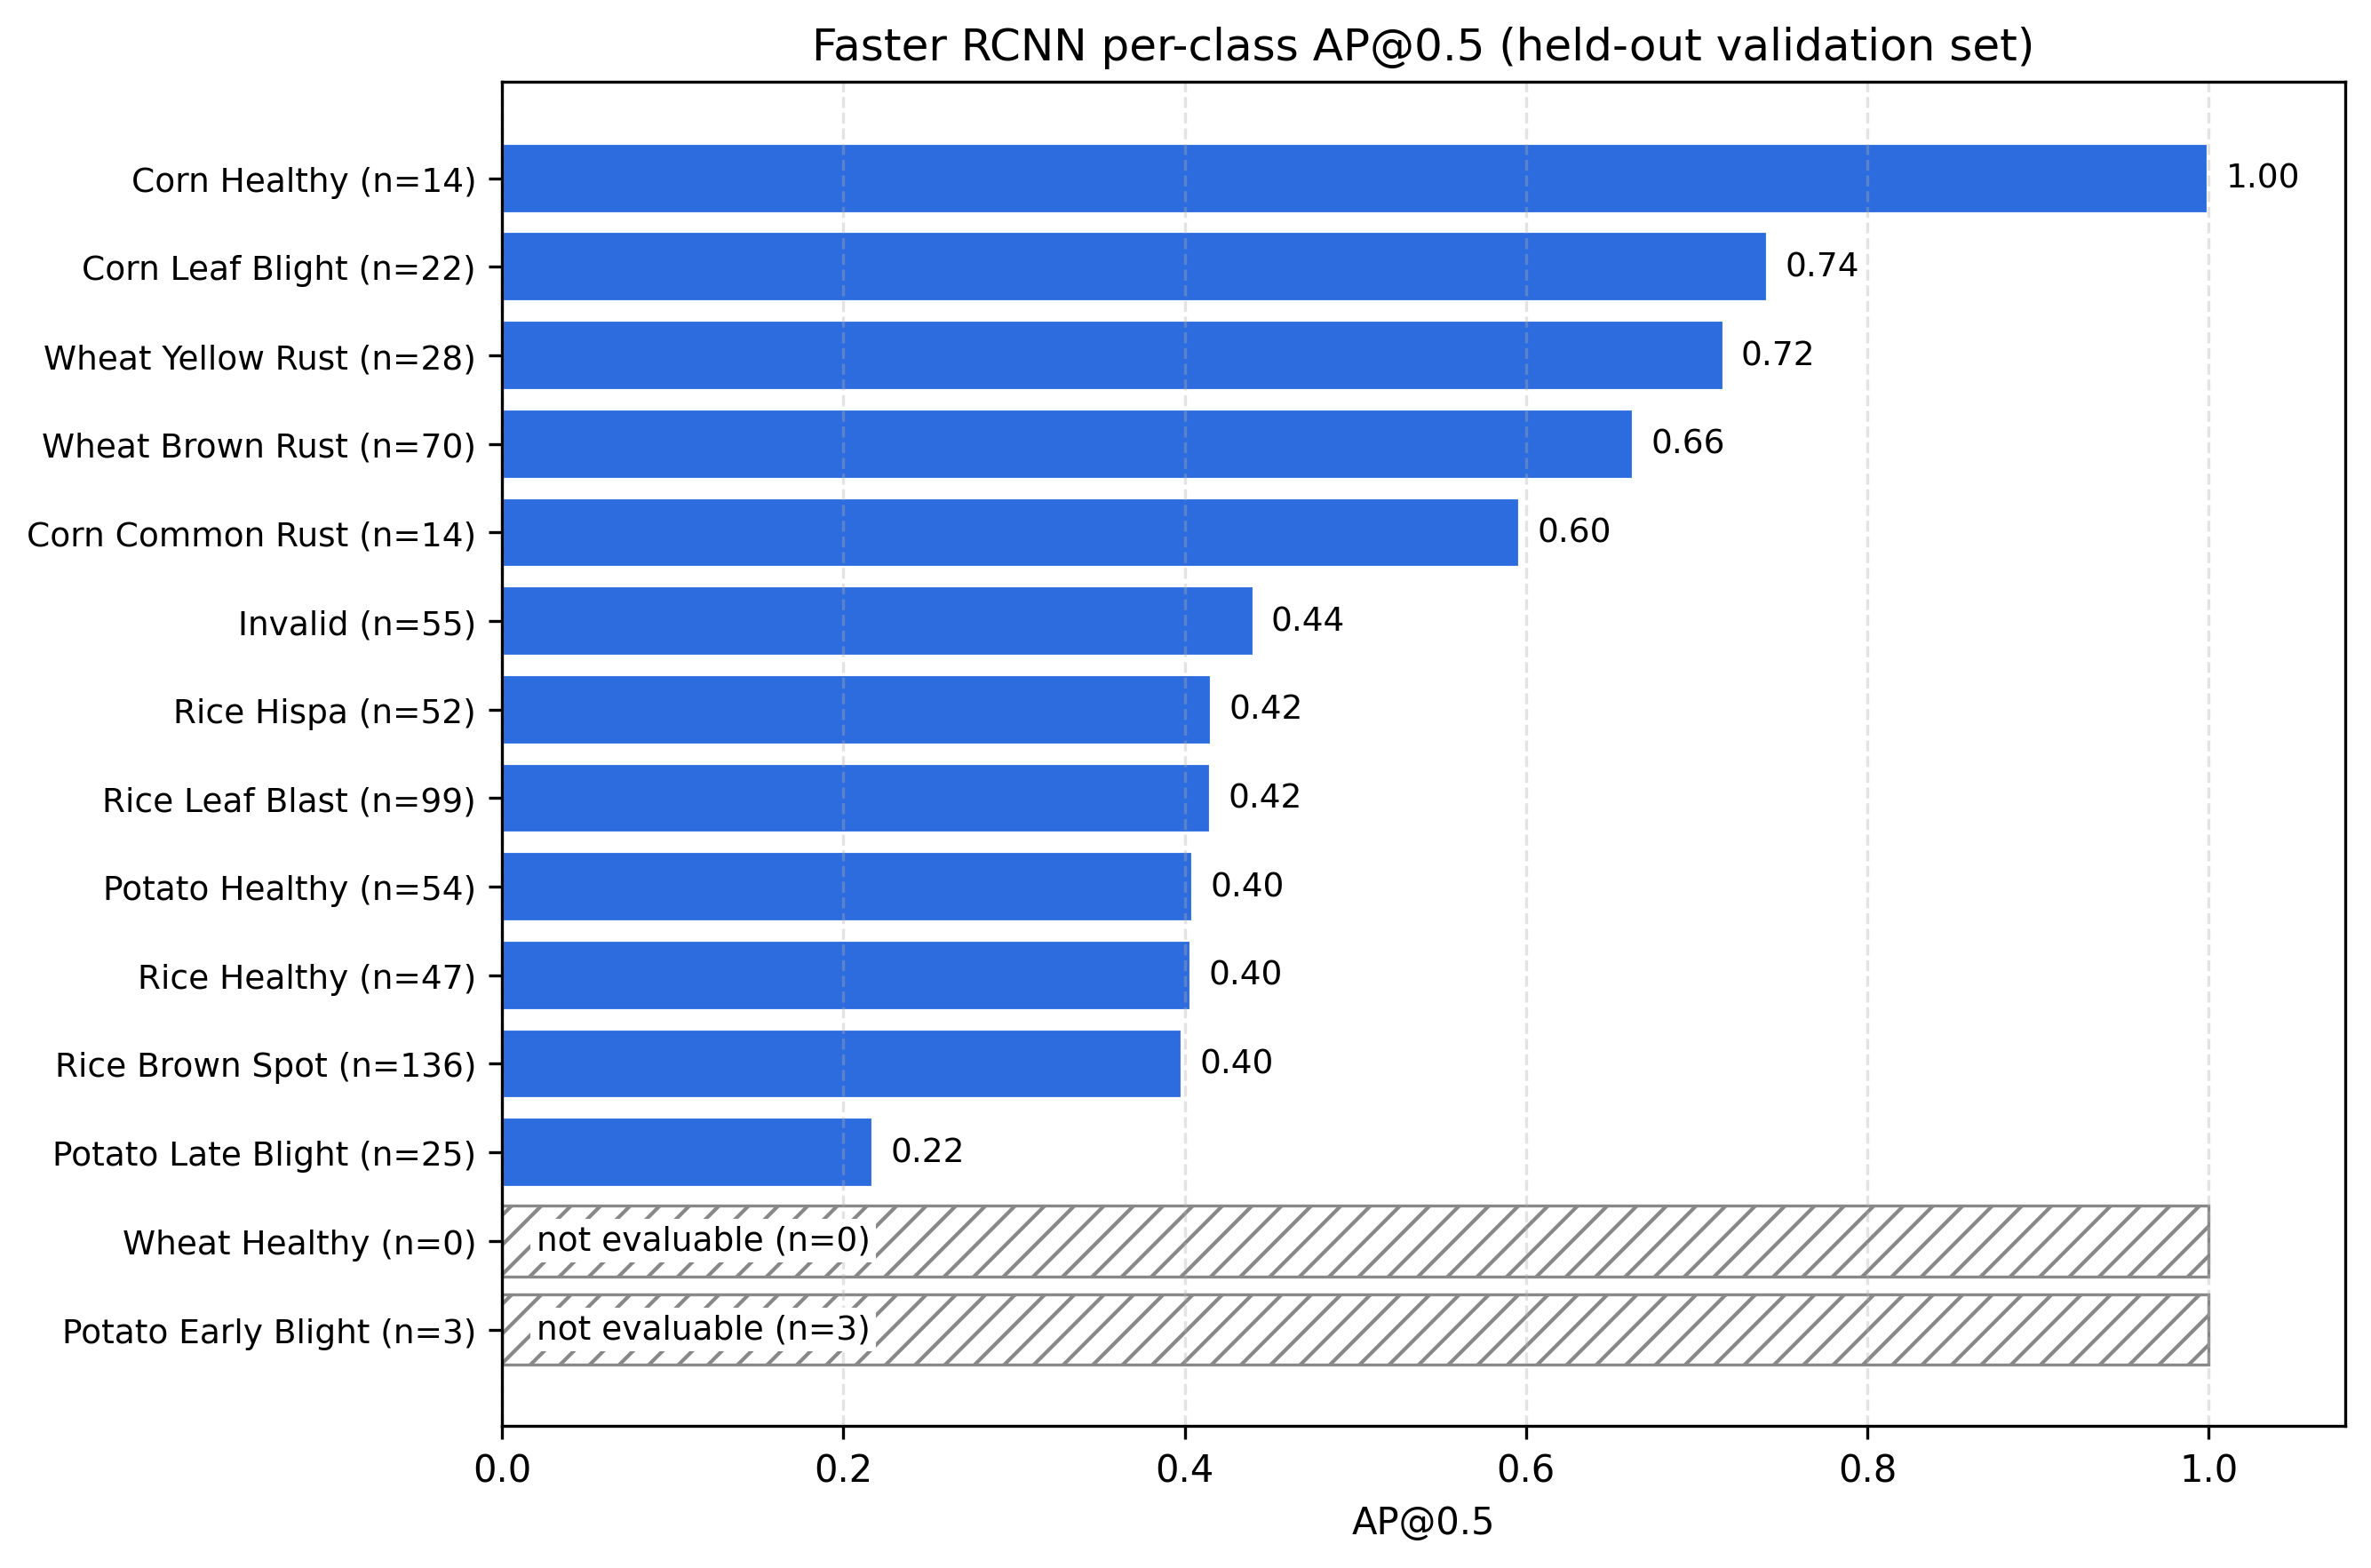
\includegraphics[width=0.9\textwidth]{figures/faster_rcnn_per_class_ap.png}
\caption{Severity-aware Faster RCNN per-class AP@0.5 on the
  held-out validation set; $n$ is the number of validation
  annotations. Potato Early Blight ($n=3$) and Wheat Healthy ($n=0$)
  could not be reliably evaluated on this split (see text) and are
  shown hatched; their zero values should be disregarded.}
\label{fig:rcnnap}
\end{figure}

Figure~\ref{fig:annotation} illustrates the Grounding DINO
annotation pipeline.
The finding generalises beyond plant disease: zero-shot
auto-annotation is a viable strategy whenever large labelled datasets
are prohibitively expensive to build manually.

\begin{figure}[!htbp]
\centering
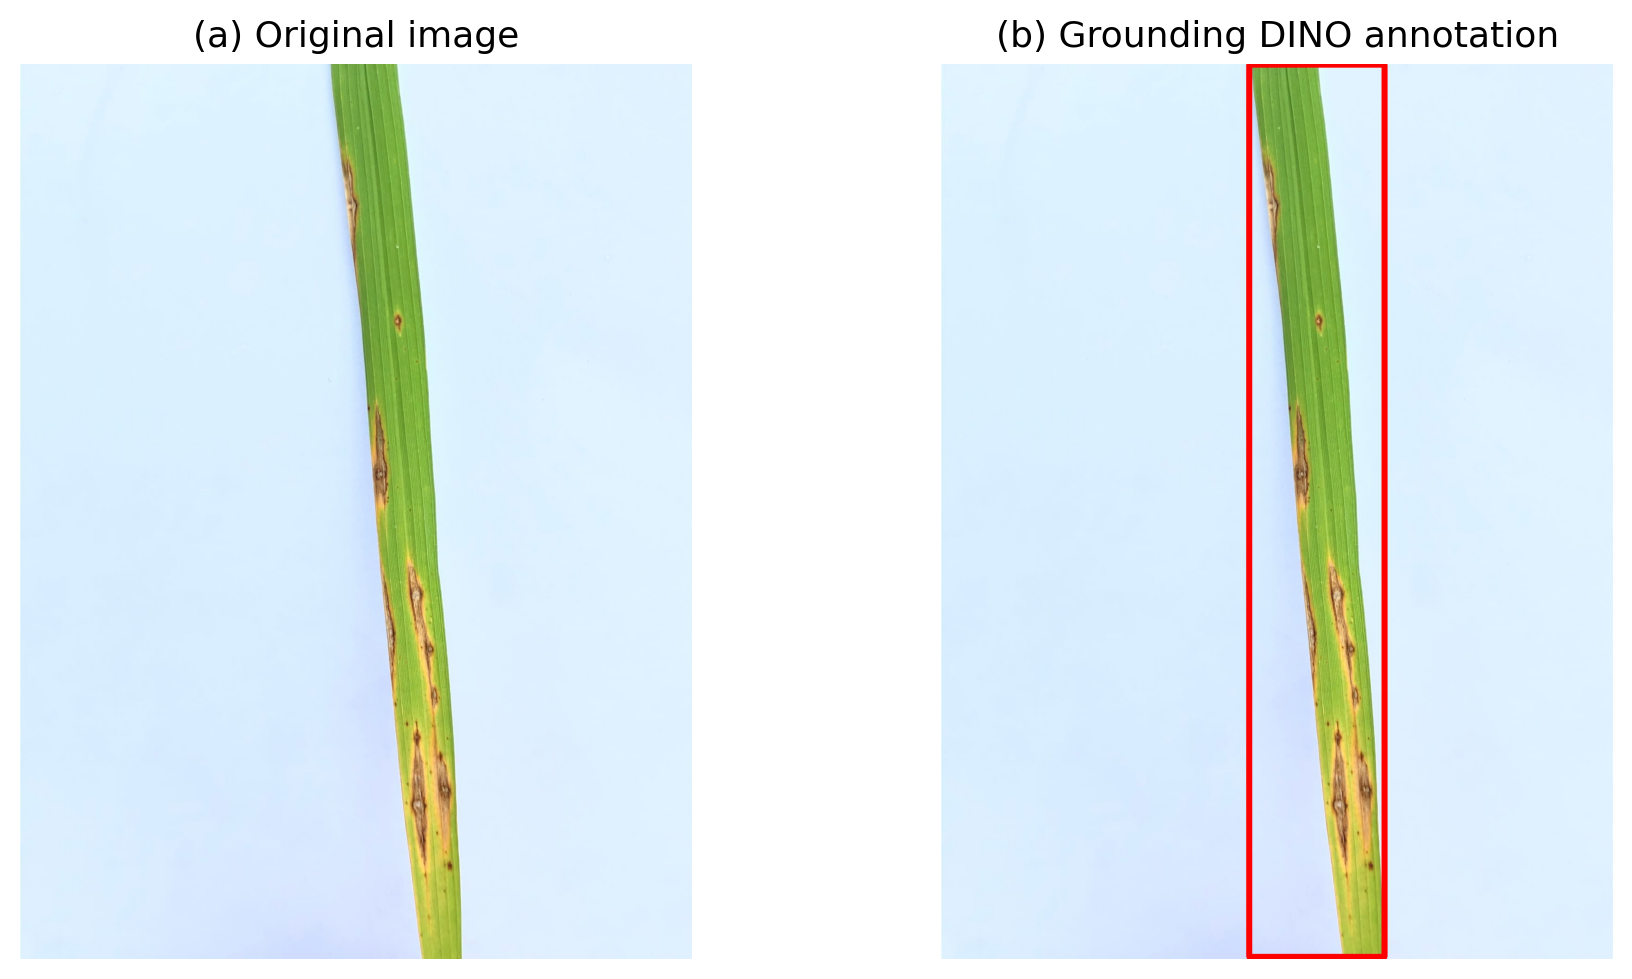
\includegraphics[width=0.55\textwidth]{figures/annotation_collage.png}
\caption{Grounding DINO zero-shot auto-annotation. Left: unlabelled
  leaf image. Right: bounding box produced automatically from the
  prompt ``disease spots on leaf'', with no manual work required.}
\label{fig:annotation}
\end{figure}

\subsection{Crop Yield Prediction (Proof of Concept)}
\label{sec:yield}

We evaluate the yield stage with a random 80/20 split of the 15,642 country-year records and with a country-held-out 5-fold \texttt{GroupKFold}, in which no country appears in both training and test folds. A crop-mean baseline predicts each crop's mean training yield and uses no features. Under the random split, every test country is also in the training set and average rainfall identifies the country, so XGBoost's R\textsuperscript{2} of 0.974 reflects memorisation of country patterns. With countries held out, XGBoost reaches $0.643 \pm 0.087$, which is no better than the crop-mean baseline ($0.637 \pm 0.095$; RMSE 52,326 versus 52,885\,hg/ha), and Random Forest ($0.573$) and Linear Regression ($0.564$) fall below it. The feature ablation in Table~\ref{tab:yield} shows the same thing: climate alone has no skill ($-0.016$), adding crop type gives $0.658$, and adding severity on top of crop type does not help ($0.643$; Random Forest changes by $-0.012$). Severity is a fixed per-crop constant with three distinct values, so it acts as a crop code and carries no disease information. Stage~3 is therefore a proof of concept of how a vision-derived severity score could be passed to a yield model. It does not show that severity improves yield prediction, which would require yield records paired with leaf images.

\begin{table}[!htbp]
\centering
\caption{Yield prediction under two evaluation protocols. Held-out =
  country-held-out 5-fold \texttt{GroupKFold} (mean $\pm$ SD over folds).
  The first four rows are the XGBoost feature ablation; the crop-mean
  baseline predicts each crop's mean training yield and uses no features.}
\label{tab:yield}
\small
\begin{tabular}{lccc}
\toprule
\textbf{Configuration} & \textbf{R\textsuperscript{2}, random} &
\textbf{R\textsuperscript{2}, held-out} & \textbf{RMSE, held-out (hg/ha)}\\
\midrule
Climate only (XGBoost)                  & $-$0.1151 & $-0.016 \pm 0.085$ & 89,808\\
Climate + crop type (XGBoost)           & 0.9699    & $0.658 \pm 0.122$  & 50,617\\
Climate + severity (XGBoost)            & 0.9606    & $0.624 \pm 0.105$  & 53,360\\
Full (climate, crop, severity), XGBoost & 0.9743    & $0.643 \pm 0.087$  & 52,326\\
\midrule
Full, Random Forest                     & 0.9789    & $0.573 \pm 0.146$  & 56,527\\
Full, Linear Regression                 & 0.6383    & $0.564 \pm 0.100$  & 58,310\\
\midrule
Crop-mean baseline                      & 0.6778    & $0.637 \pm 0.095$  & 52,885\\
\bottomrule
\end{tabular}
\end{table}

\subsection{Dynamic Severity Validation}
\label{sec:results_dynamic}

% NOTE: this entire section was recomputed with substantial bug fixes.
% The computation previously (a) never actually loaded the trained
% Faster RCNN -- it used a generic, off-the-shelf COCO-pretrained
% detector instead; (b) used an outdated 14-class list missing
% Corn Gray Leaf Spot; (c) counted "Healthy"-category boxes as lesion
% area, inflating healthy-class severity; and (d) summed overlapping
% boxes from different predicted categories without deduplication,
% producing lesion ratios exceeding 1.0 (physically impossible). All
% four issues are fixed below: the actual trained detector is used,
% the class list is corrected, Healthy/Invalid boxes are excluded from
% the lesion-area sum, and lesion area is computed as the true pixel
% union of remaining boxes.
Applying Equation~\ref{eq:dynamic_severity} to 15 images per class
from the detection dataset, using the \textbf{actual trained}
severity-aware Faster RCNN and EfficientNetV2S classifier, yielded the
computed scores in Table~\ref{tab:dynamic_severity}.

\begin{table}[!htbp]
\centering
\caption{Dynamic severity scores computed from the trained Faster RCNN
  and EfficientNetV2S confidence ($n = 15$ images per class,
  confidence threshold = 0.4), compared with fixed literature values.
  Std = standard deviation.}
\label{tab:dynamic_severity}
\setlength{\tabcolsep}{5pt}
{\small
\begin{tabular}{lccc}
\toprule
\textbf{Disease Class} & \textbf{Literature} &
\textbf{Computed Mean} & \textbf{Computed Std}\\
\midrule
Corn Common Rust    & 0.35 & 0.0000$^{*}$ & 0.0000\\
Corn Gray Leaf Spot & n/a$^{\ddagger}$ & 0.1044 & 0.2858\\
Corn Healthy        & 0.00 & 0.0086 & 0.0331\\
Corn Leaf Blight    & 0.40 & 0.8570 & 0.1348\\
Potato Early Blight & 0.20 & 0.0000$^{\dagger}$ & 0.0000\\
Potato Healthy      & 0.00 & 0.0006 & 0.0024\\
Potato Late Blight  & 0.45 & 0.0000$^{\dagger}$ & 0.0000\\
Rice Brown Spot     & 0.25 & 0.4060 & 0.2112\\
Rice Healthy        & 0.00 & 0.0648 & 0.1747\\
Rice Hispa          & 0.30 & 0.1044 & 0.2359\\
Rice Leaf Blast     & 0.50 & 0.1728 & 0.1819\\
Wheat Brown Rust    & 0.35 & 0.4681 & 0.4620\\
Wheat Healthy       & 0.00 & 0.1718 & 0.3411\\
Wheat Yellow Rust   & 0.40 & 0.3610 & 0.4639\\
\bottomrule
\end{tabular}
}
\\[4pt]
\footnotesize $^{*}$Threshold-boundary artifact, not a genuine zero
(see discussion below). $^{\dagger}$Reflects a genuine detector
confusion pattern, not a threshold artifact (see discussion below).
$^{\ddagger}$No literature severity estimate was available for Corn Gray
Leaf Spot. The detector was not trained on this class
(Section~\ref{sec:detection}), so this row reflects detections from
other categories.
\end{table}

Two findings stand out beyond the general small-lesion
under-estimation pattern already discussed in Section~3.3.1.

\textbf{Threshold sensitivity (Corn Common Rust).} At the standard
0.4 confidence threshold, Corn Common Rust scores a computed severity
of 0.0000; unthresholded inspection shows the model's top (correct)
prediction scores 0.31 to 0.32, just below the cutoff. Testing a lower
threshold (0.3) recovers Corn Common Rust but introduces a new
problem: false-positive lesion area on Rice Healthy images, whose
computed severity rises to 0.48. A single global confidence threshold
cannot simultaneously suit all classes; per-class calibration is
noted as future work.

\textbf{A genuine detector weakness (Potato classes).} Diseased
Potato Early Blight and Late Blight images are frequently
misclassified by the detector as Potato Healthy with high confidence
(0.52 to 0.88), a pattern that persists even at a lower confidence
threshold, confirming it is not a calibration artifact. This traces
to severe class imbalance in the detection training annotations:
Potato Healthy has 245 annotations versus Potato Early Blight's 29.
This is a distinct weakness from the small-lesion under-counting
behaviour discussed in Section~3.3.1, and is noted as a specific
limitation warranting targeted class rebalancing in future work.

Beyond these two specific findings: Rice Brown Spot (computed 0.406
vs.\ literature 0.25) and Wheat Brown Rust (computed 0.468 vs.\
literature 0.35) show the closest overall agreement, supporting the
detection-based approach for classes with large, clearly defined
lesions. Rice Hispa and Rice Leaf Blast remain underestimated relative
to literature, consistent with the Grounding DINO small-lesion
under-counting behaviour identified in Section~3.3.1.
Taken together, these findings support the feasibility of
image-derived severity estimation while identifying a
plant-disease-specific detector as the key next step.

\subsection{PlantVillage Overlap Check}\label{sec:plantvillage}
We evaluated ConvNeXtLarge on the potato images of the publicly available PlantVillage dataset (2,152 images; the PlantVillage download available to us contained only Pepper, Potato and Tomato crops). Using the model's full 15-class output, it classified 99.91\% of them correctly, with two errors (both Potato Late Blight predicted as Potato Healthy). This is not independent validation. A hash comparison showed that every one of these 2,152 images is also present in our dataset: 4,304 files in the potato classes are byte-identical to the 2,152 PlantVillage potato images. The potato classes of the Bangladeshi dataset therefore appear to be PlantVillage images, which, together with the duplicate analysis in Section~\ref{sec:split}, helps explain why they are classified almost perfectly. Many corn files also carry PlantVillage-style names (for example \texttt{RS\_Rust 1576}); we could not test this because the available PlantVillage download did not include corn. Independent validation requires a dataset with no shared provenance and is left to future work.

\subsection{Web Interface Demo}

\begin{figure}[!htbp]
\centering
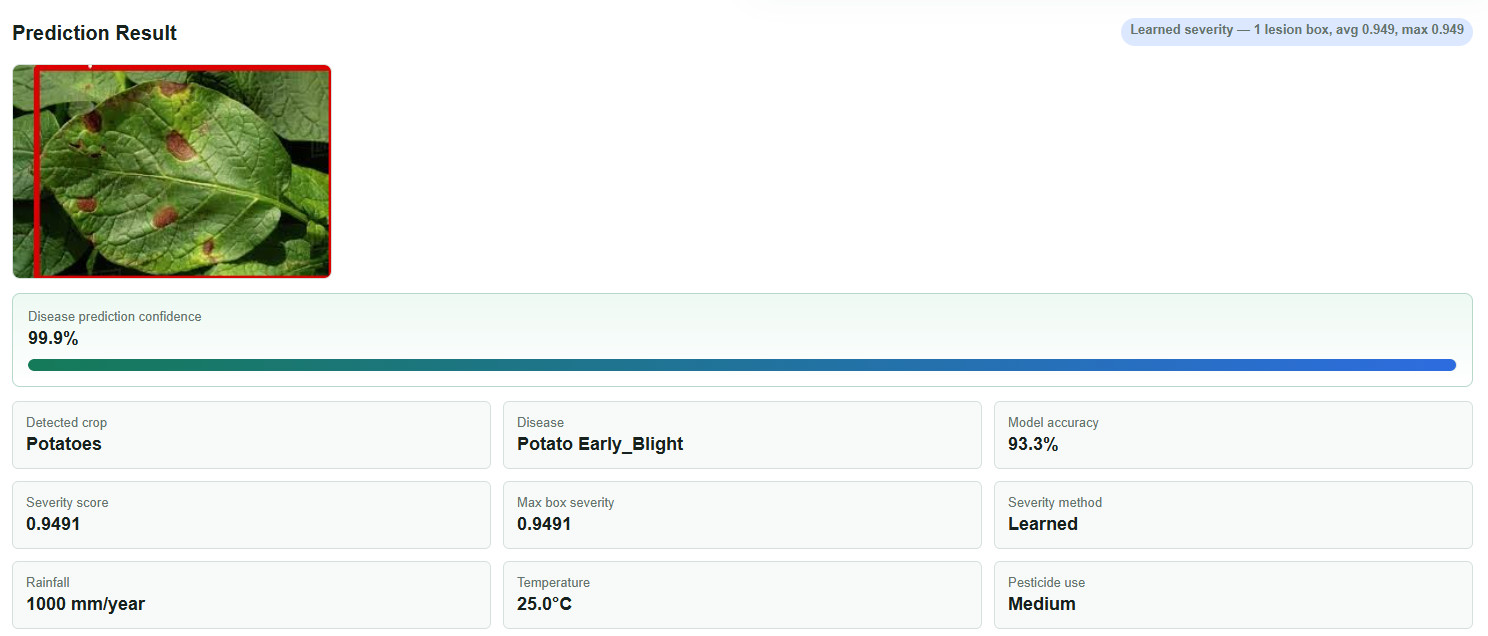
\includegraphics[width=0.95\textwidth]{figures/web_interface.png}
\caption{Demonstration of the pipeline interface. A potato leaf
  image is classified as Potato Early Blight at 99.9\% confidence by
  EfficientNetV2S, and the severity-aware Faster RCNN returns a single
  lesion box spanning most of the image, with a learned severity of 0.95.
  This illustrates the single-box-per-image behaviour discussed in
  Section~\ref{sec:detection}: the score overstates the visible lesion
  coverage. The yield tiles are omitted because the yield model has no
  demonstrated skill beyond crop identity (Section~\ref{sec:yield}); the
  figure illustrates the interface only.}
\label{fig:demo}
\end{figure}

\subsection{Model Explainability}

\subsubsection{Grad-CAM Visualisation.}
\label{sec:gradcam_full}
We generated Grad-CAM heatmaps for three correctly classified and
three misclassified images of \textbf{ConvNeXtLarge}, a top-group
model (Figure~\ref{fig:gradcam}); the examples were drawn from the dataset
and were not restricted to the test split.
For correctly classified images, the activation maps consistently
highlight the diseased tissue: rust pustules on Corn Common Rust,
lesion texture on Corn Gray Leaf Spot, and the uniform green surface
for Corn Healthy.
The misclassified cases confirm the \textbf{bidirectional} confusion
between Rice Hispa and Rice Healthy identified in
Section~\ref{sec:perclass} (19 of 78 Rice Hispa images misclassified
as Rice Healthy; 13 of 78 Rice Healthy images misclassified as Rice
Hispa).
The heatmaps show that the model attends to minor textural
irregularities on the leaf surface in both directions of confusion.

These visualisations matter beyond illustration. For growers and
extension officers to act on an automated diagnosis, they need
evidence that the prediction rests on lesion tissue rather than on
background, leaf edges or acquisition artefacts~\cite{selvaraju2017};
Grad-CAM makes such shortcut learning detectable, and the confusion
cases here show that the errors arise from genuinely ambiguous surface
texture rather than from spurious cues.

\begin{figure}[!htbp]
\centering
\begin{subfigure}[b]{0.32\textwidth}
  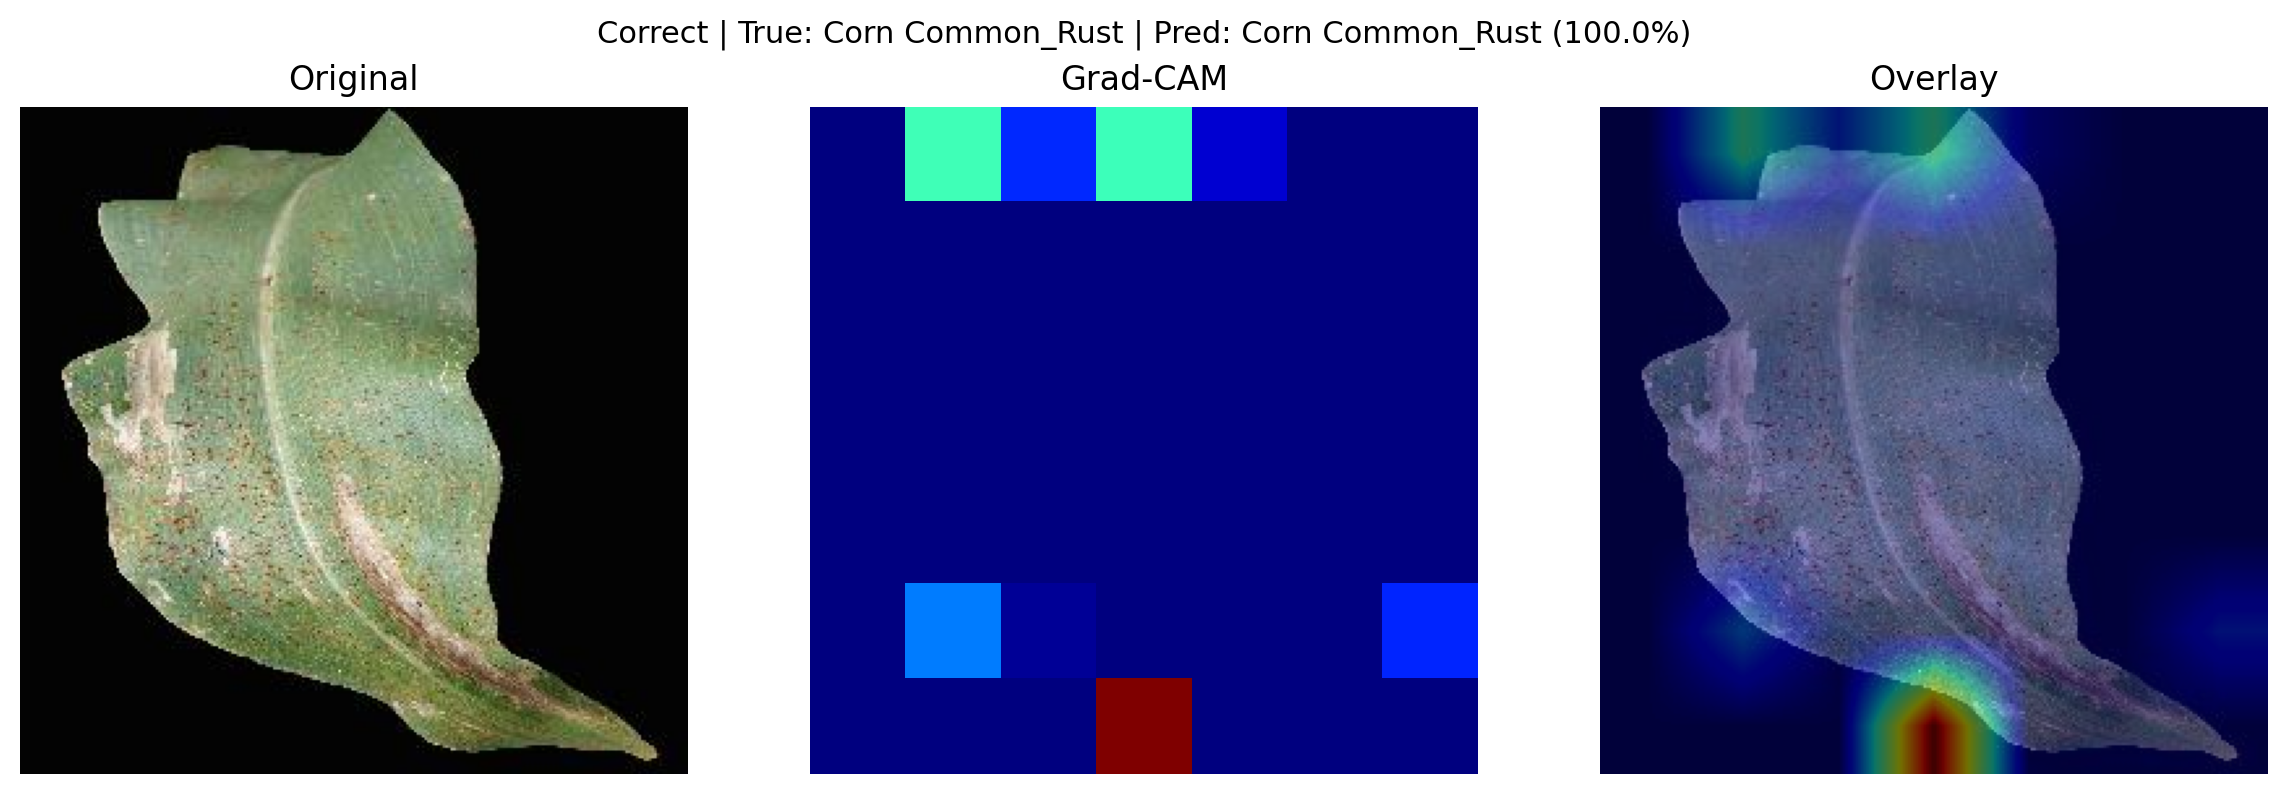
\includegraphics[width=\textwidth]{figures/01_correct_Corn___Common_Rust_pred_Corn___Common_Rust.png}
  \caption{Correct: Corn Common Rust}
\end{subfigure}
\hfill
\begin{subfigure}[b]{0.32\textwidth}
  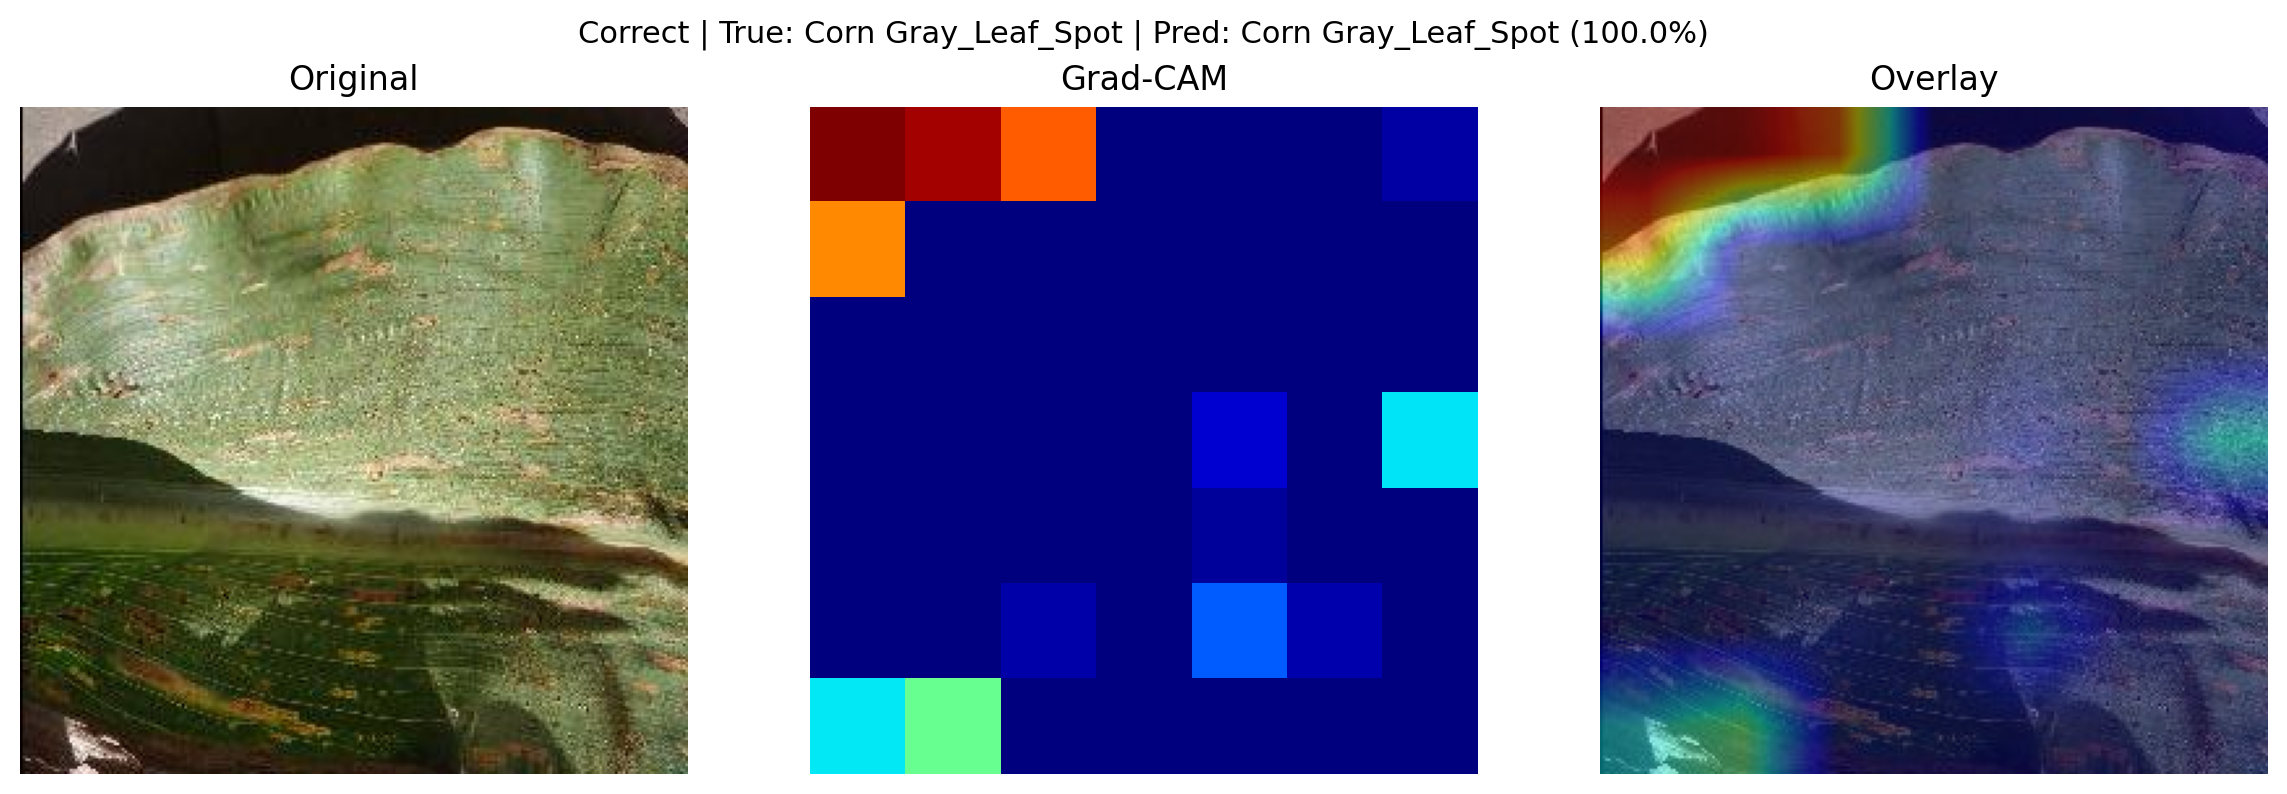
\includegraphics[width=\textwidth]{figures/02_correct_Corn___Gray_Leaf_Spot_pred_Corn___Gray_Leaf_Spot.png}
  \caption{Correct: Corn Gray Leaf Spot}
\end{subfigure}
\hfill
\begin{subfigure}[b]{0.32\textwidth}
  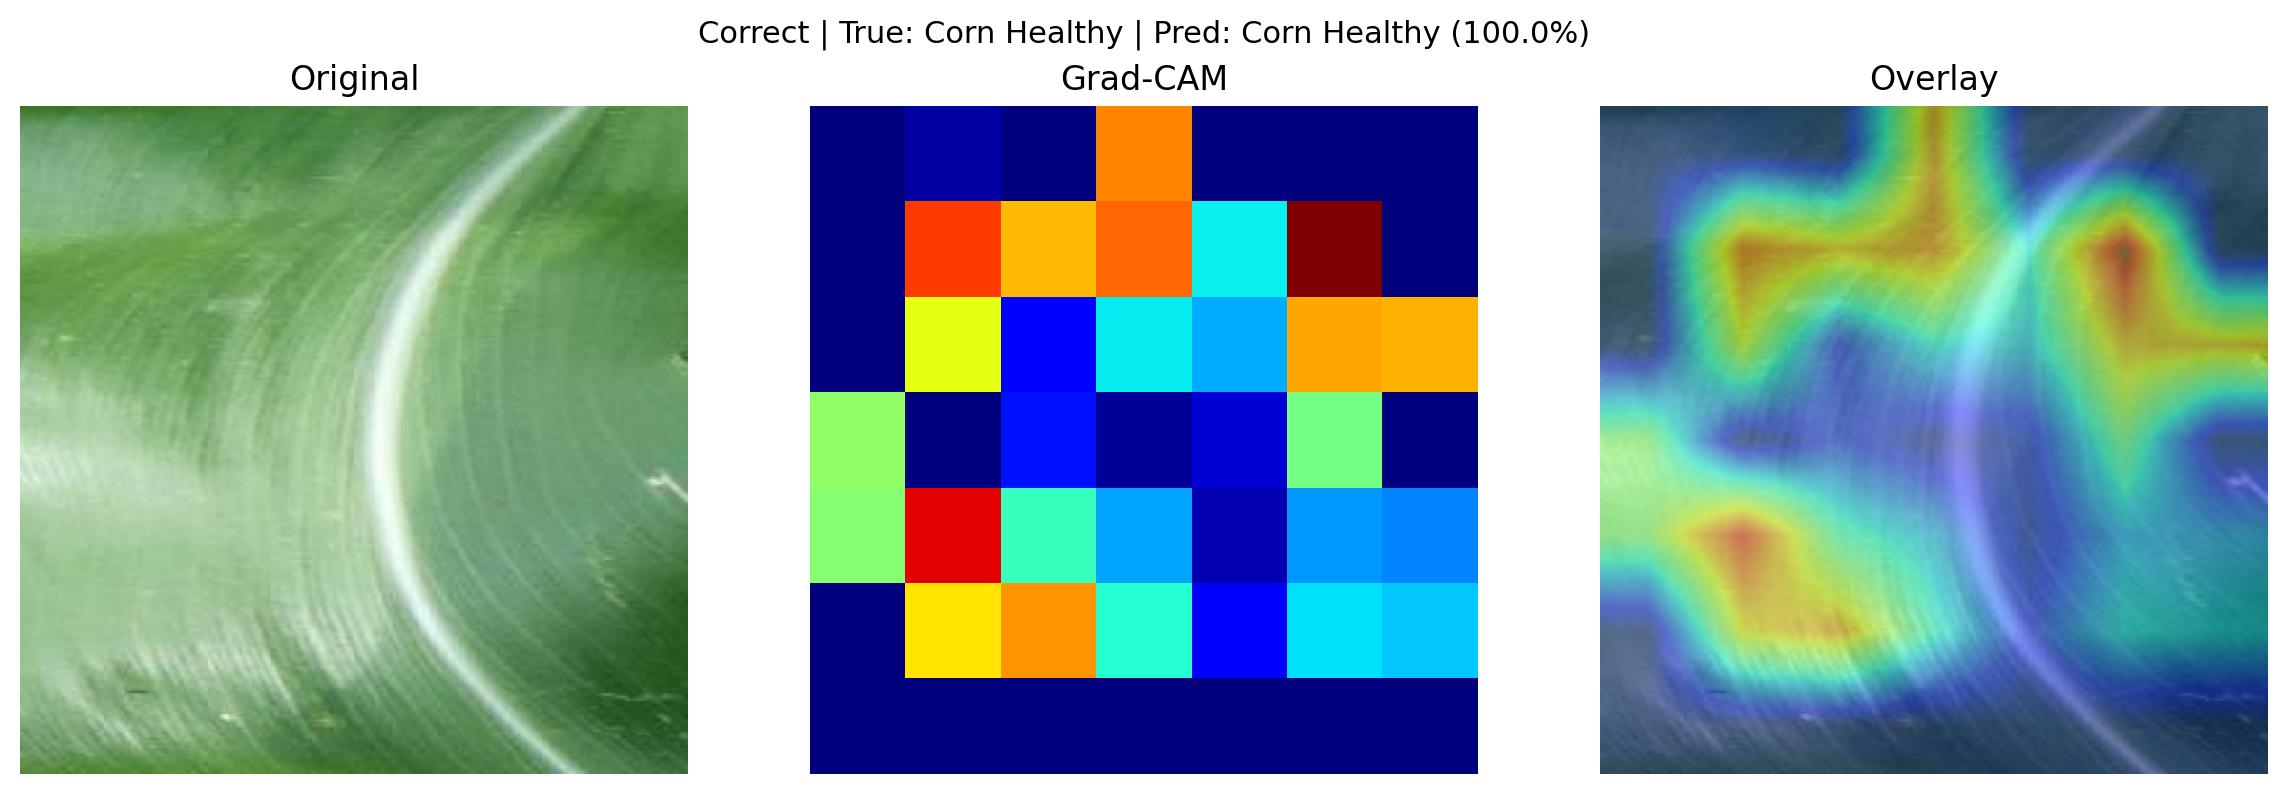
\includegraphics[width=\textwidth]{figures/03_correct_Corn___Healthy_pred_Corn___Healthy.png}
  \caption{Correct: Corn Healthy}
\end{subfigure}
\vspace{0.4cm}
\begin{subfigure}[b]{0.32\textwidth}
  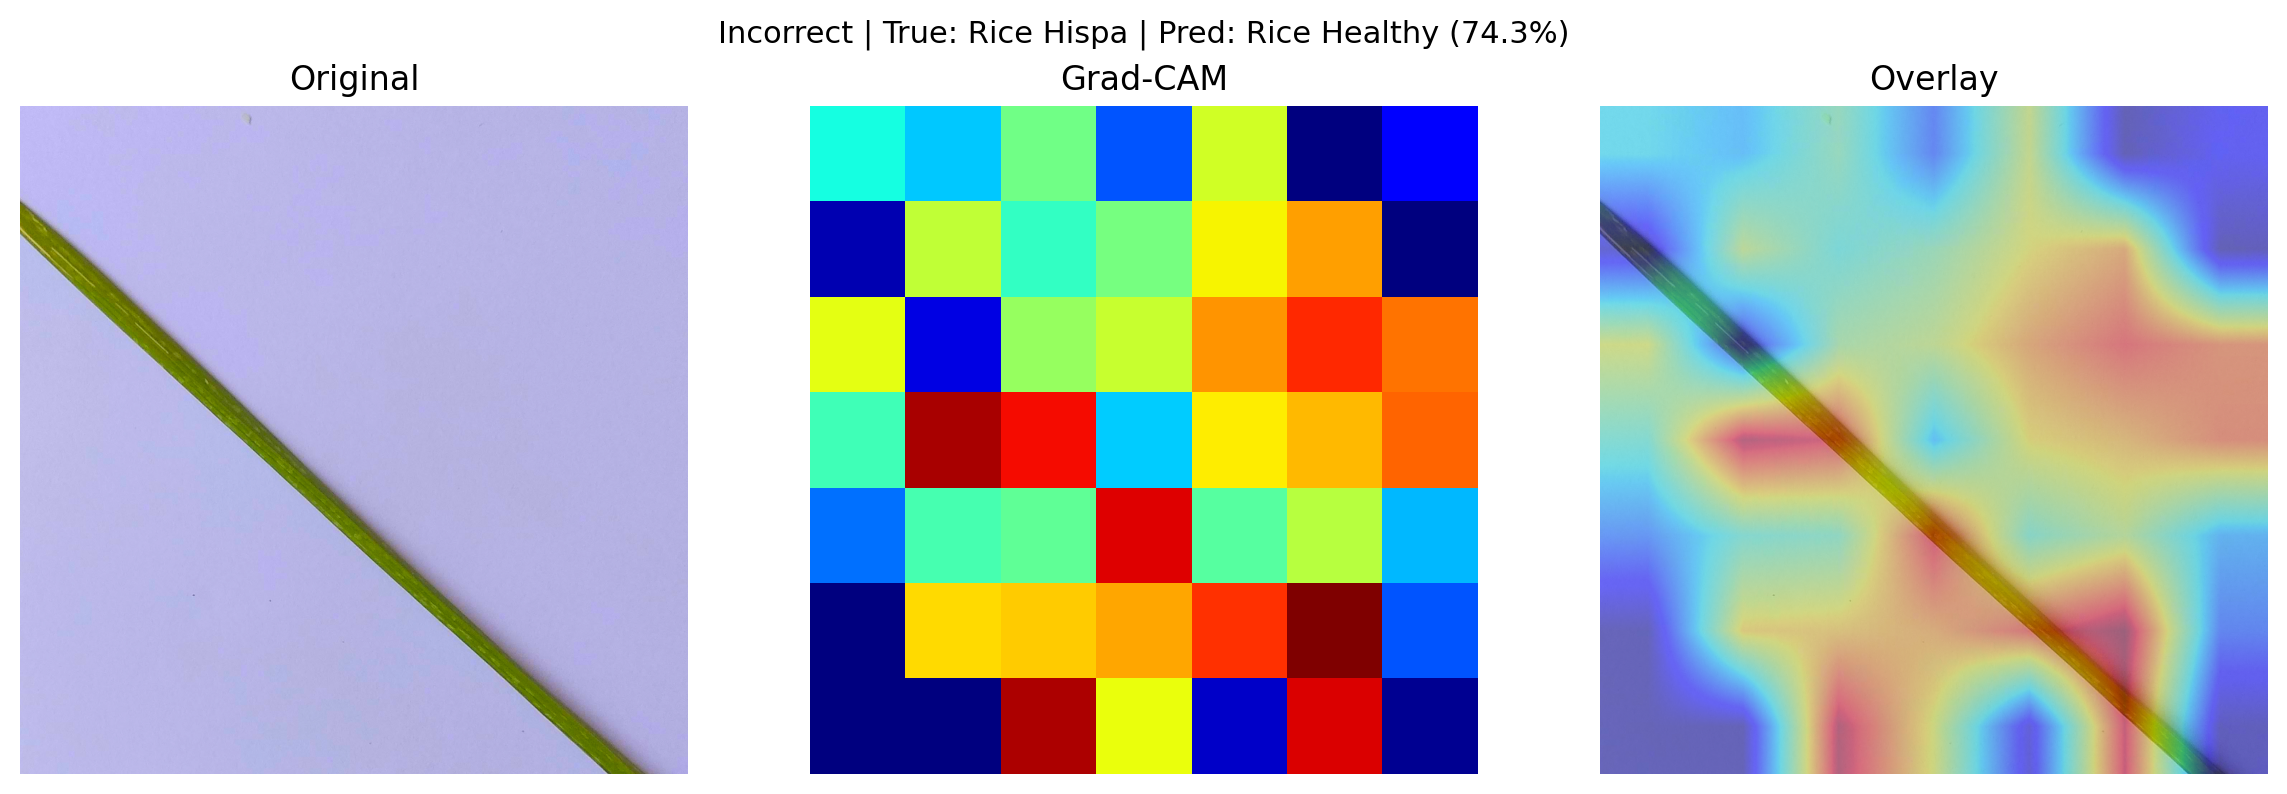
\includegraphics[width=\textwidth]{figures/04_incorrect_Rice___Hispa_pred_Rice___Healthy.png}
  \caption{Wrong: Rice Hispa $\to$ Healthy}
\end{subfigure}
\hfill
\begin{subfigure}[b]{0.32\textwidth}
  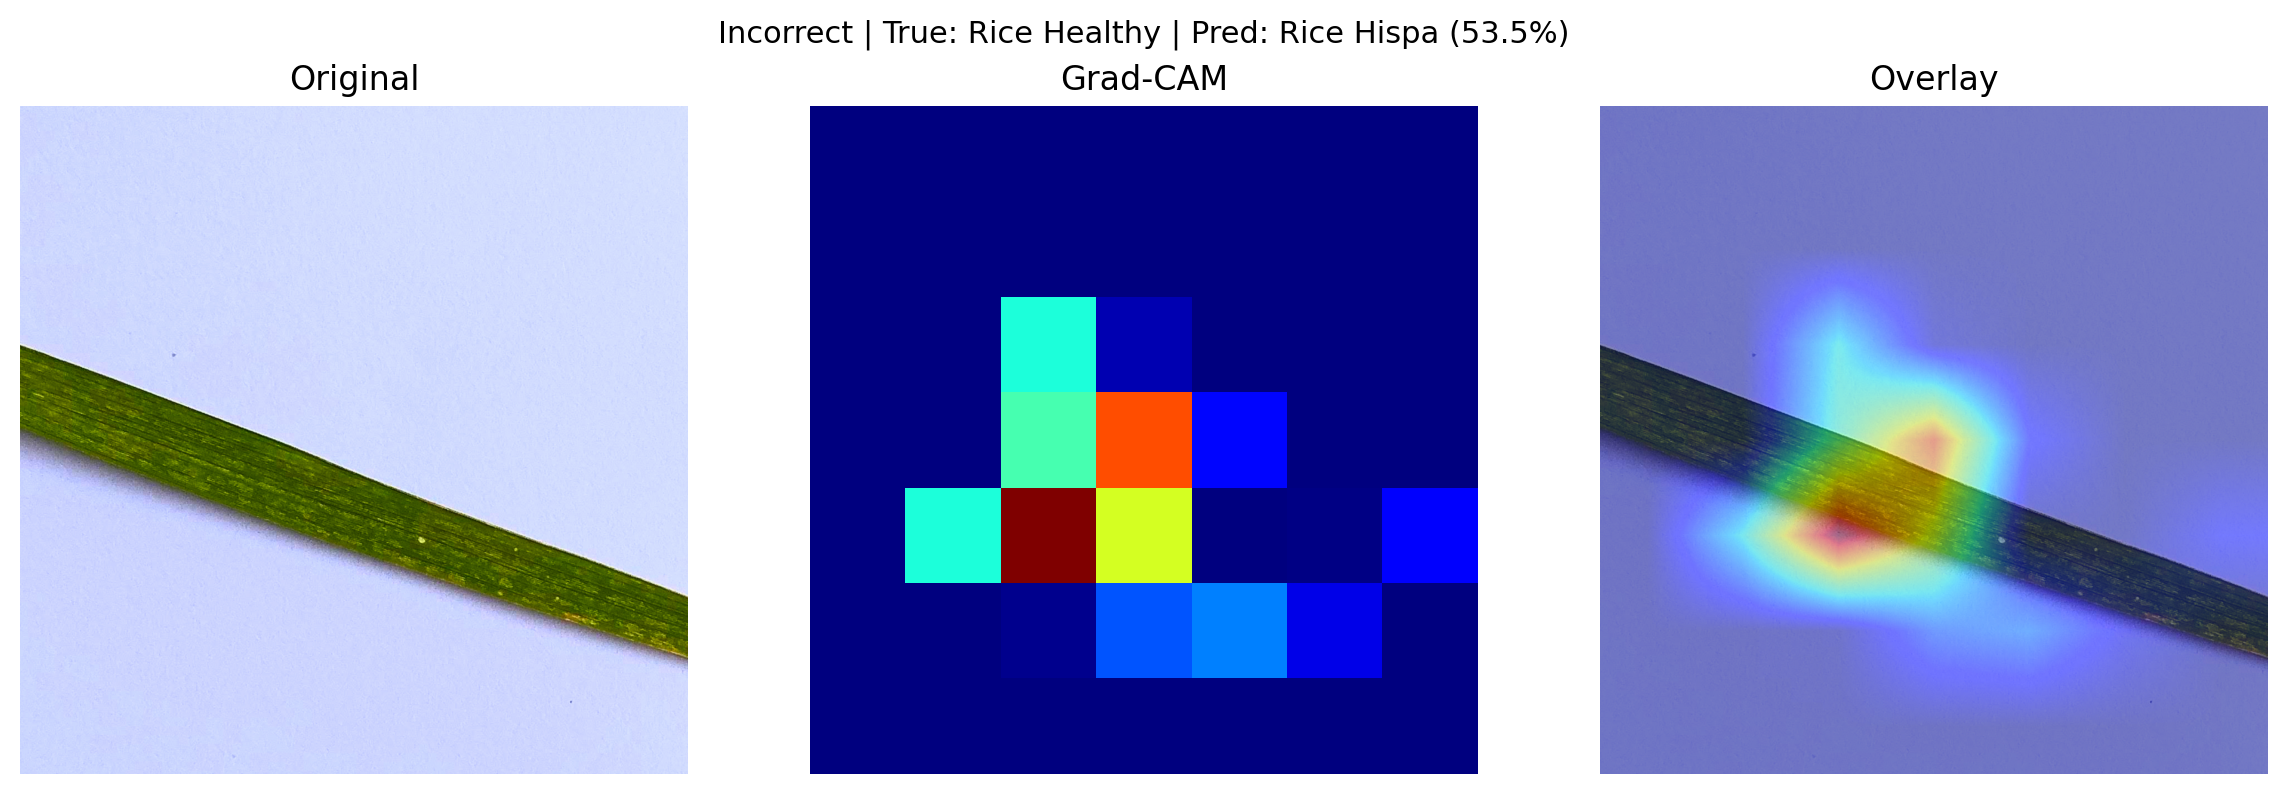
\includegraphics[width=\textwidth]{figures/05_incorrect_Rice___Healthy_pred_Rice___Hispa.png}
  \caption{Wrong: Rice Healthy $\to$ Hispa}
\end{subfigure}
\hfill
\begin{subfigure}[b]{0.32\textwidth}
  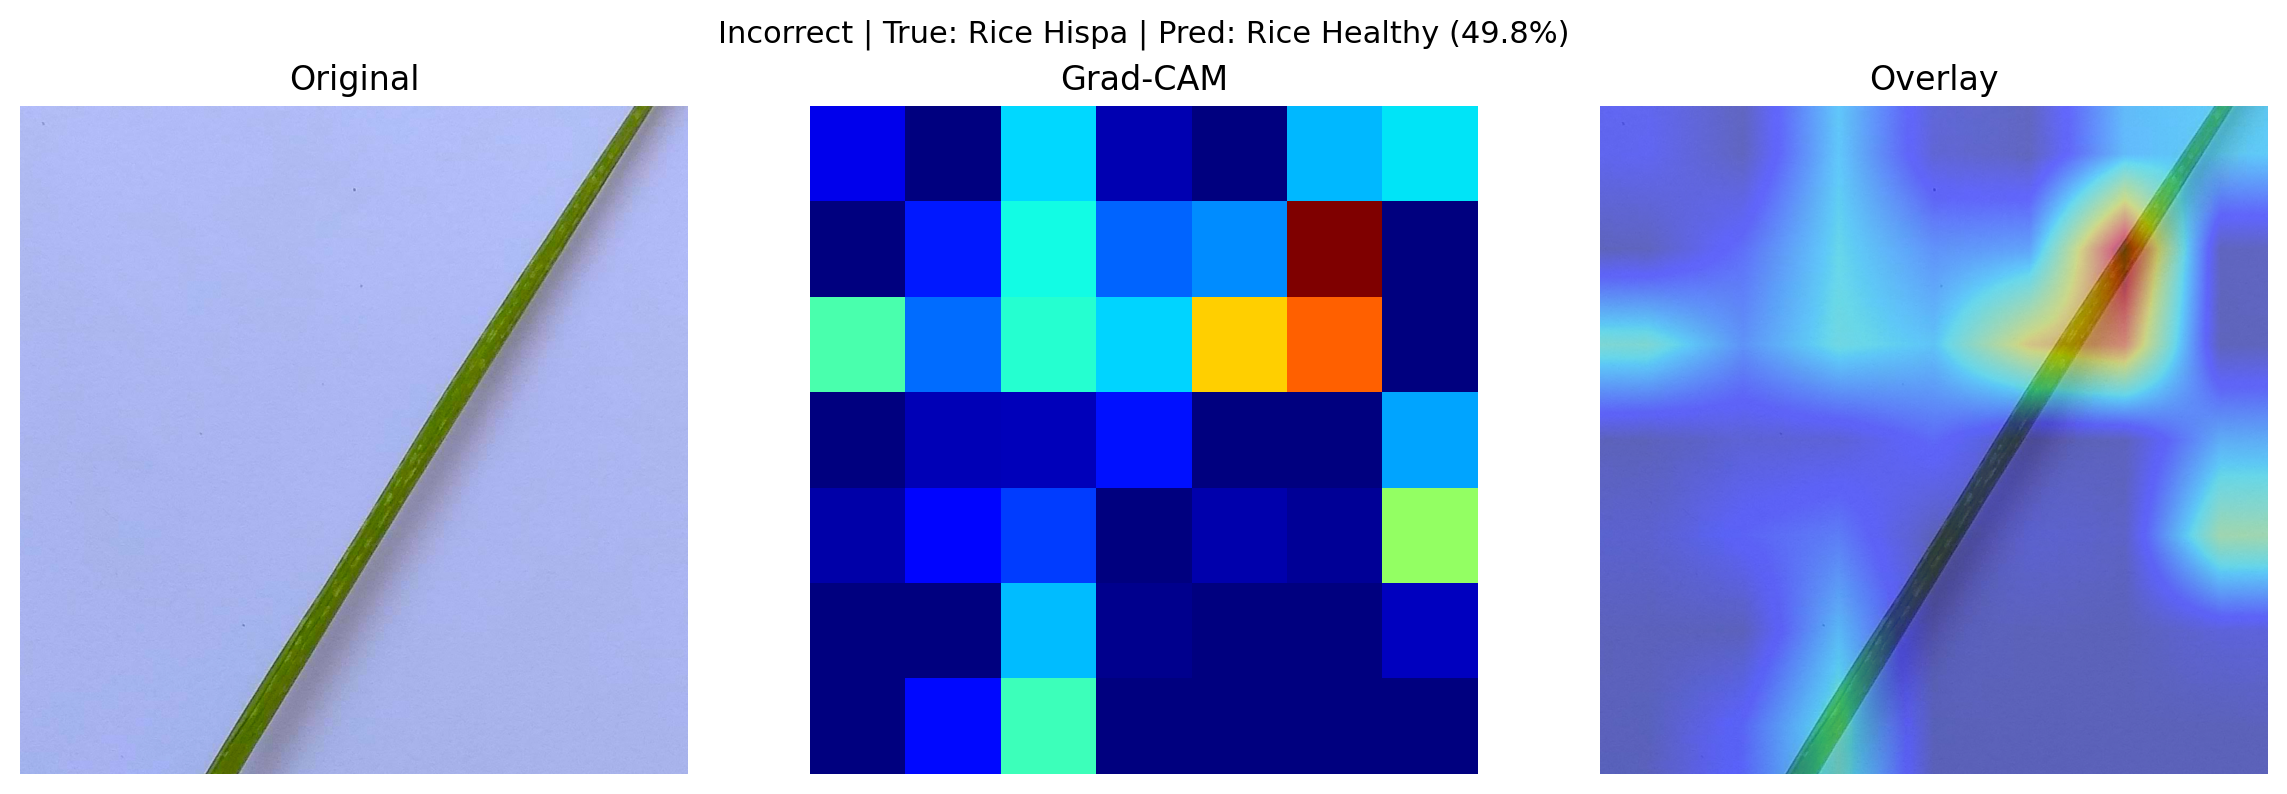
\includegraphics[width=\textwidth]{figures/06_incorrect_Rice___Hispa_pred_Rice___Healthy.png}
  \caption{Wrong: Rice Hispa $\to$ Healthy}
\end{subfigure}
\caption{Grad-CAM heatmaps for ConvNeXtLarge. Top row: correct predictions where activation maps focus on the diseased leaf tissue. Bottom row: bidirectional Rice Hispa/Healthy misclassifications; the model responds to surface irregularities that mimic the opposite class in both directions.}
\label{fig:gradcam}
\end{figure}

\subsubsection{SHAP Diagnostic of the Yield Model.}
Figure~\ref{fig:shap} shows SHAP plots for the XGBoost yield model. \texttt{disease\_severity} has the highest mean absolute SHAP value, but its dependence plot shows only three vertical clusters (0.217, 0.25 and 0.26), one per crop-level constant, so the plots reflect crop identity and not disease: potatoes carry the lowest severity code and the highest typical yield. We draw no agronomic conclusion from them. They are kept as a diagnostic that exposed the confound described in Section~\ref{sec:yield}.

\begin{figure}[!htbp]
\centering
\begin{subfigure}[b]{0.48\textwidth}
  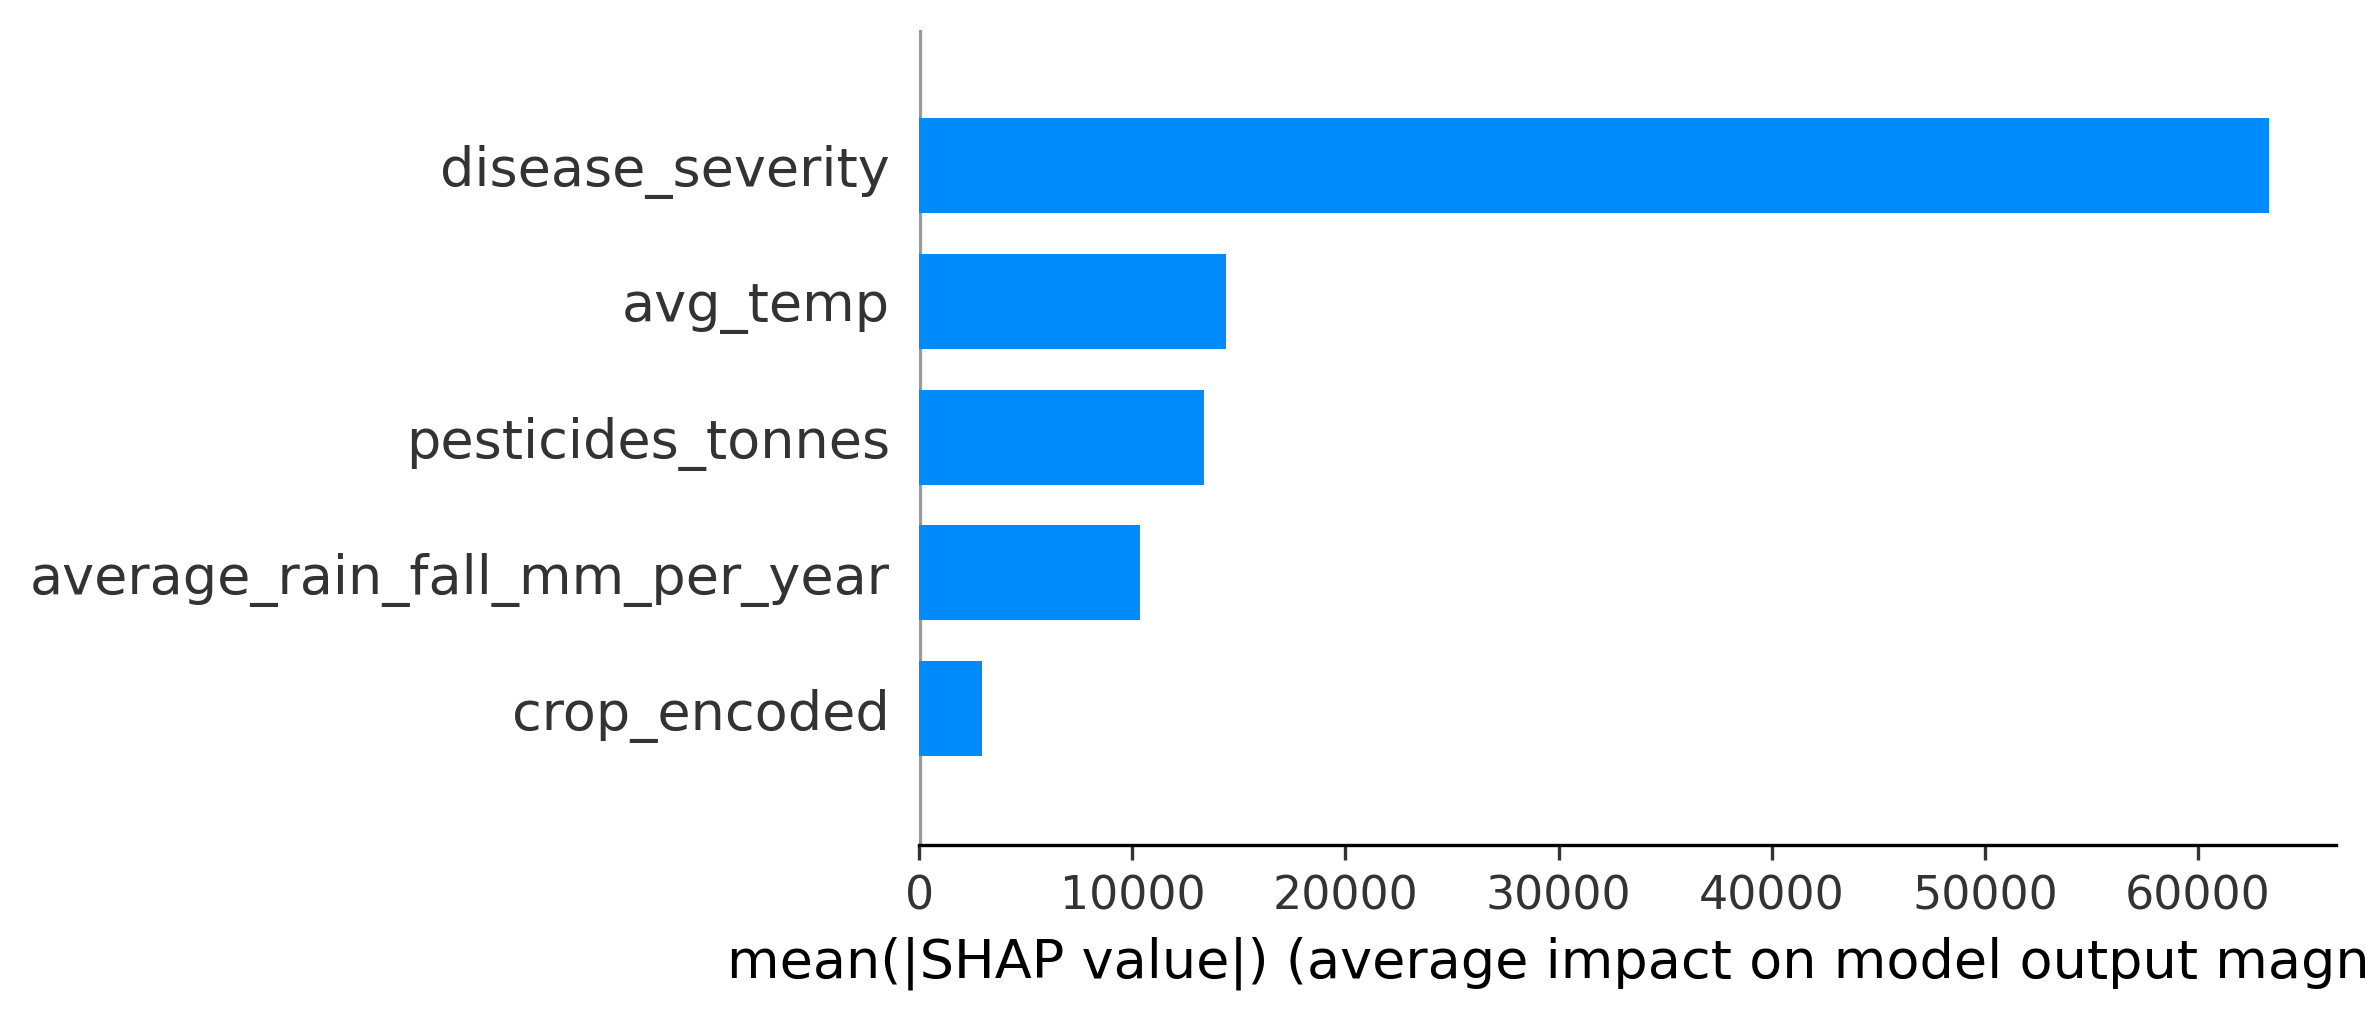
\includegraphics[width=\textwidth]{figures/shap_summary_bar.png}
  \caption{Mean absolute SHAP values per feature}
\end{subfigure}
\hfill
\begin{subfigure}[b]{0.48\textwidth}
  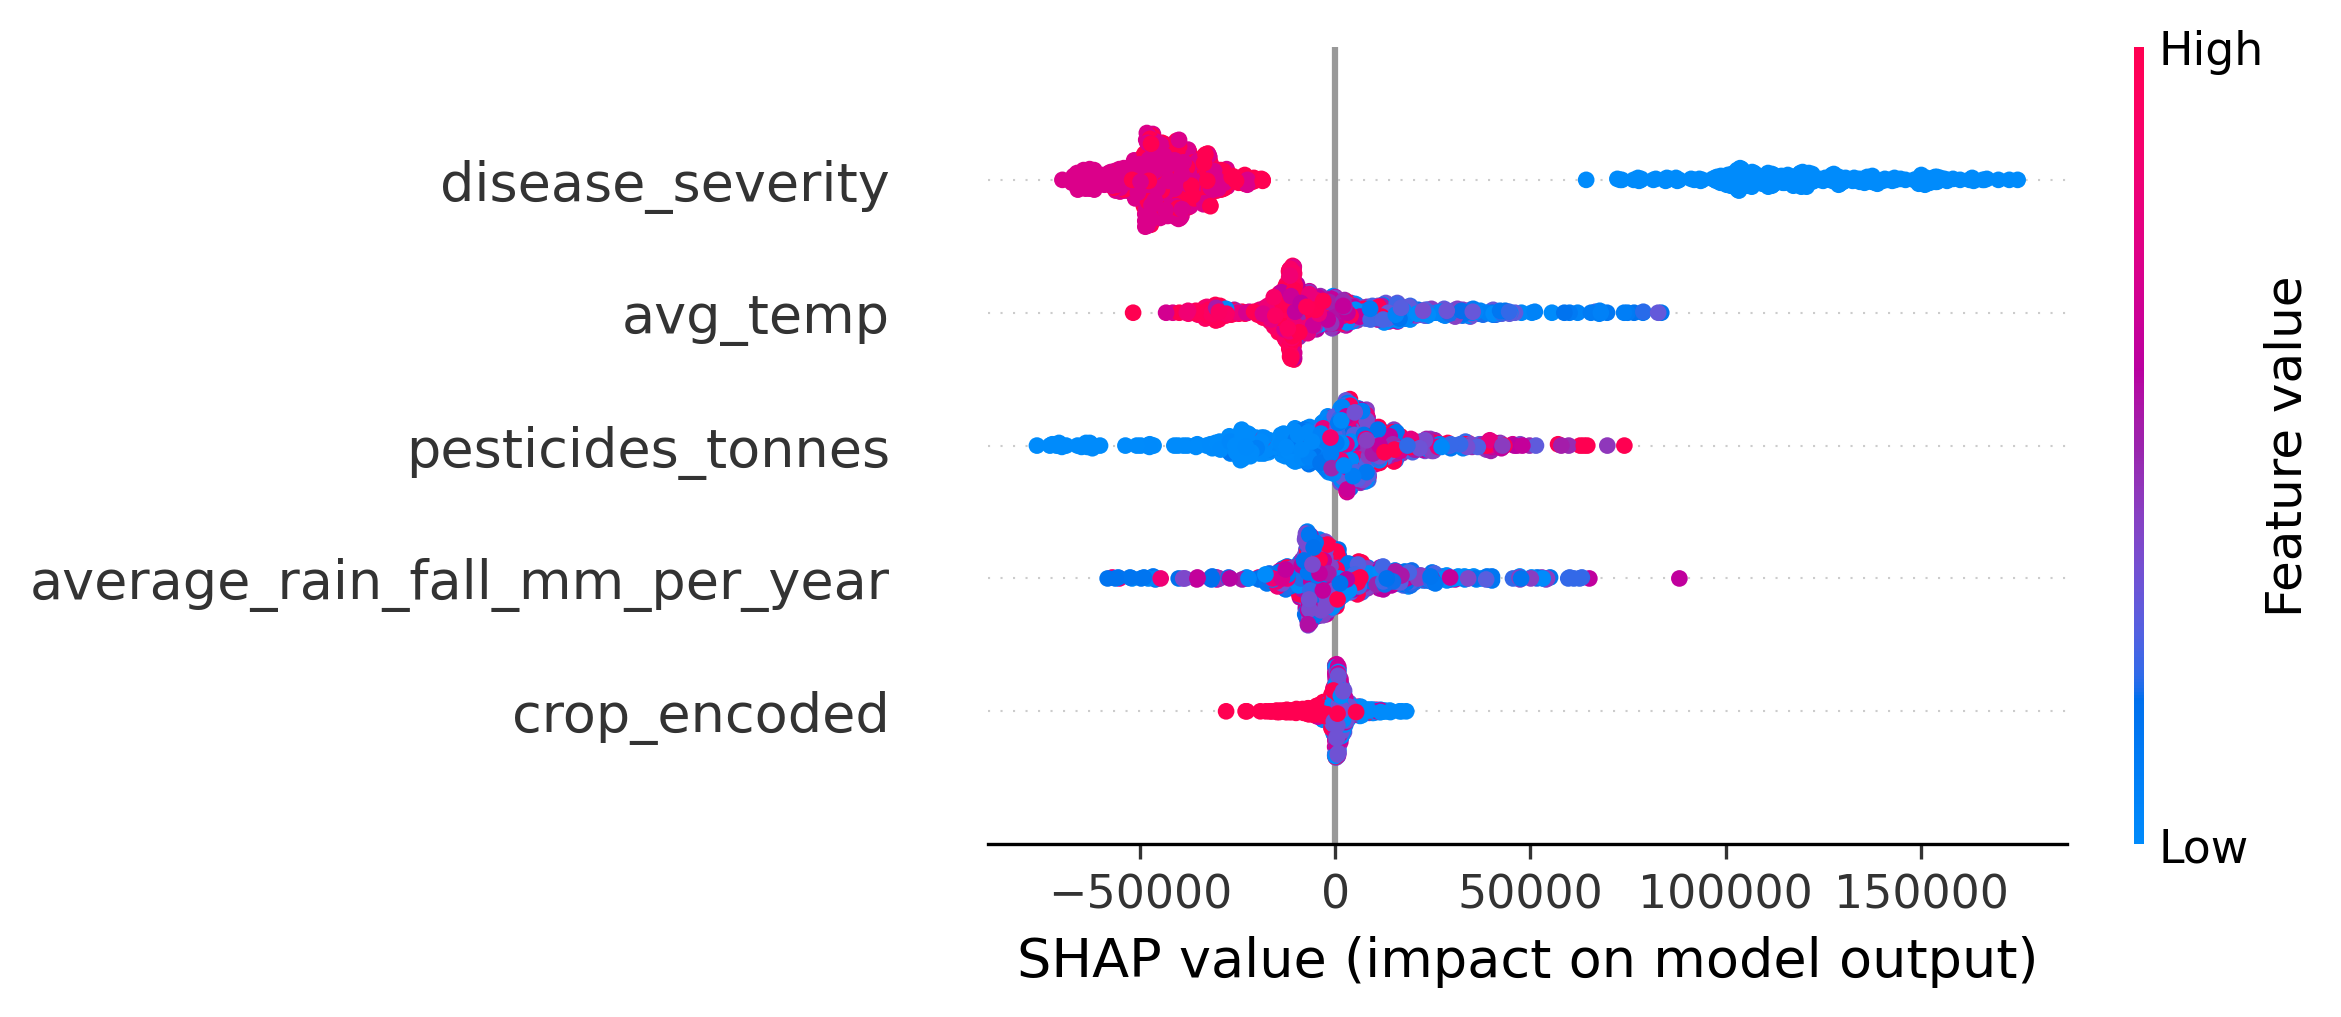
\includegraphics[width=\textwidth]{figures/shap_summary_beeswarm.png}
  \caption{SHAP beeswarm plot}
\end{subfigure}
\vspace{0.4cm}
\begin{subfigure}[b]{0.65\textwidth}
  \centering
  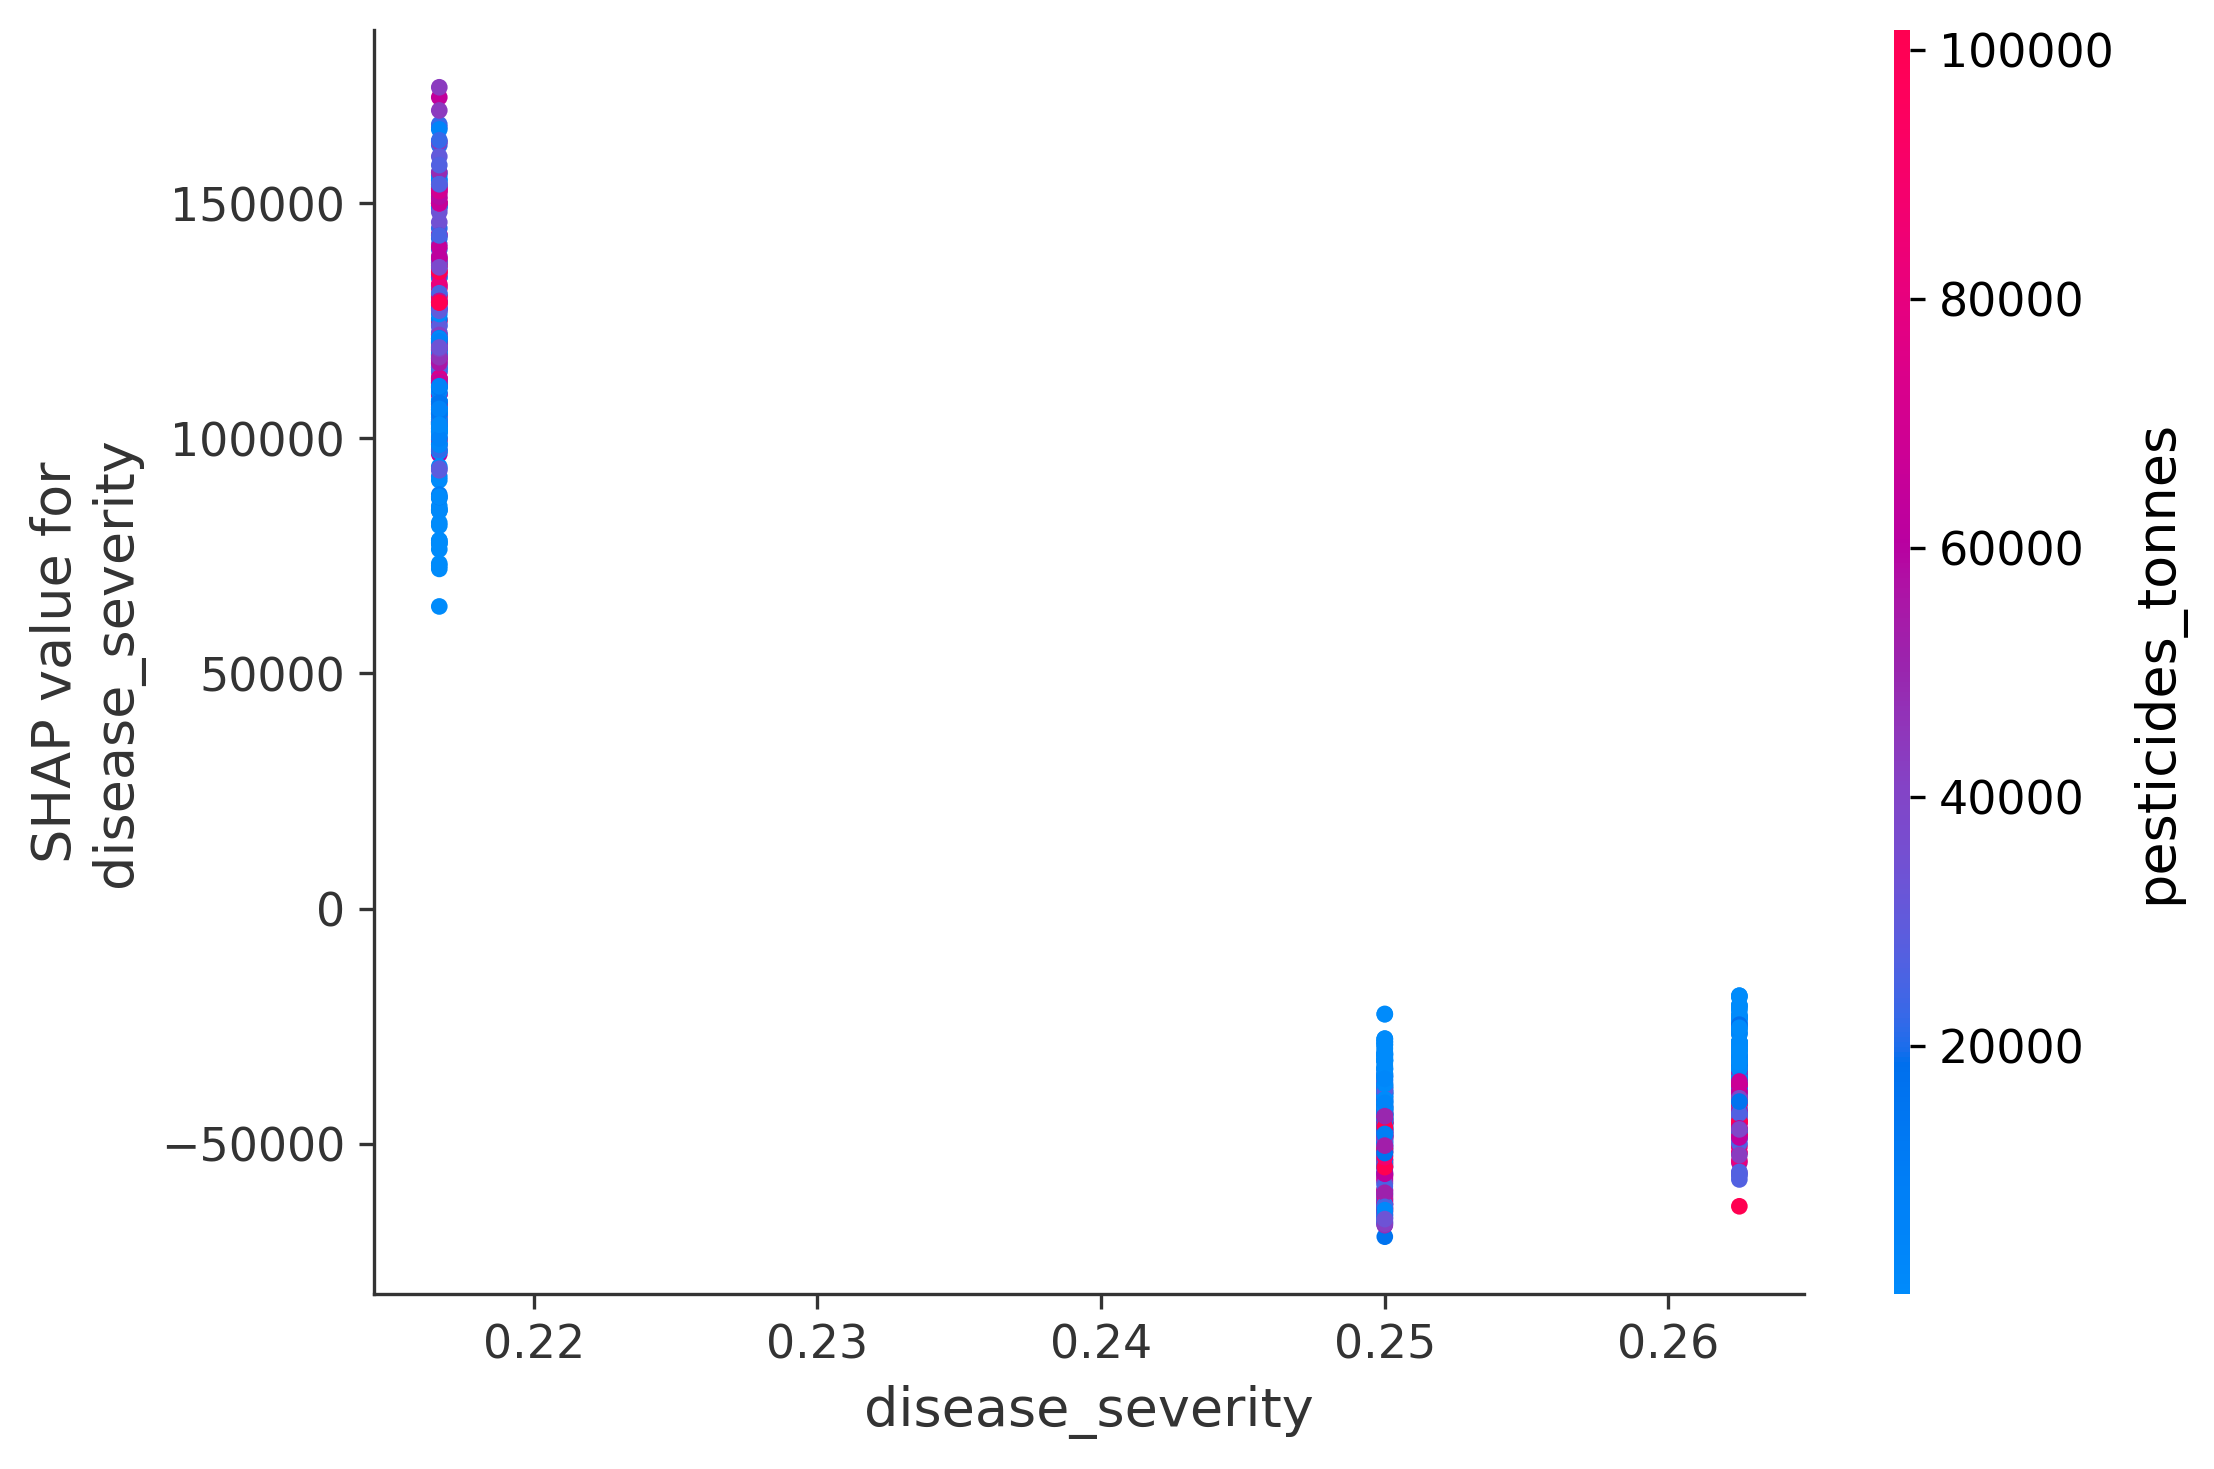
\includegraphics[width=\textwidth]
    {figures/shap_dependence_disease_severity.png}
  \caption{SHAP dependence plot for \texttt{disease\_severity}}
\end{subfigure}
\caption{SHAP diagnostic of the XGBoost yield model.
  (a) \texttt{disease\_severity} has the highest mean absolute SHAP
  value. (b) Beeswarm plot. (c) The dependence plot shows three
  clusters, one per crop-level constant: the feature acts as a crop
  code, so these plots reflect crop identity, not disease.}
\label{fig:shap}
\end{figure}

\subsection{Limitations}
\label{sec:limitations}

The limitations below fall into two groups. Those in the first group prevent the framework from being validated as a whole; those in the second limit how far individual results can be generalised.

\textbf{A. Limitations that prevent full validation}
\begin{enumerate}[noitemsep]
  \item \textbf{Unmatched datasets.} FAO yield records and Bangladeshi
    leaf images are not matched by location or season. The pipeline is
    validated on proxy data rather than a properly paired dataset.
  \item \textbf{The yield stage shows no skill beyond crop identity.}
    Severity is a fixed per-crop constant in training (three distinct
    values), and with countries held out XGBoost
    (R\textsuperscript{2} = 0.64) does not outperform a crop-mean
    baseline (0.64); the random-split R\textsuperscript{2} of 0.97 is
    inflated by country overlap. No conclusion about severity's value
    for yield prediction can be drawn from this dataset.
  \item \textbf{No leaf-to-field aggregation.} Severity is computed
    per leaf photograph; the sampling and aggregation needed to obtain
    a field-level indicator were not implemented or tested
    (Section~\ref{sec:stage3}).
  \item \textbf{Duplicates in the training data.} About 30\% of the dataset's files are exact copies of another file. The models were trained on a split that still contained duplicate pairs across training and validation, and were not retrained after the audit; only the evaluation was de-duplicated. Retraining on a hash-grouped split is left to future work. As a result, checkpoint selection used a validation set that shares duplicates with the training set, and duplicated images carry extra weight in training. The de-duplicated test subset protects the evaluation but not the training, so the ranking of models could change after retraining on a hash-grouped split.
  \item \textbf{Unvalidated severity labels.} Severity targets are
    computed from automatically generated Grounding DINO boxes and, like
    the literature proxies, have not been validated by an agronomist, so
    the learned severity head inherits the annotation pipeline's biases,
    notably single-box under-counting.
  \item \textbf{Severity head.} The head was trained for 5 epochs with
    a frozen backbone on 1,850 images, and its MAE of 0.2206 is measured
    against Grounding DINO coverage targets rather than manual
    annotations, so its error against true lesion coverage is unknown
    and is likely to be larger for small or numerous lesions.
  \item \textbf{Small-lesion detection and annotation under-counting.}
    Detection mAP@0.5:0.95 is 0.104 for small objects versus 0.388 for
    large regions, and Grounding DINO frequently returns a single box
    per image regardless of the true lesion count
    (Section~\ref{sec:detection}), limiting recall and dynamic
    severity accuracy for multi-lesion classes.
  \item \textbf{Manual annotations not held out.} The manually
    annotated images form part of the pool used to train and validate
    the Faster RCNN rather than an independent human-verified test set.
    A controlled ablation (manual-only, pseudo-only, manual plus
    pseudo, and severity head) against a fixed held-out manual set is
    deferred to future work because of the additional training runs it
    requires.
  \item \textbf{Non-uniform training protocol.} Fine-tuning was reserved 
  for the larger backbones, so the three mobile models 
  (MobileNet, MobileNetV2, NASNetMobile) were trained with a frozen 
  backbone only; ConvNeXtLarge and ConvNeXtXLarge, the two largest 
  models, were also left frozen to limit compute and training time. 
  The other 33 models had their last 10 backbone layers fine-tuned.
  Differences between a frozen and a fine-tuned model therefore mix 
  the effect of the architecture with that of the training procedure, 
  and we draw no conclusions from such comparisons. In particular, 
  ConvNeXtLarge and ConvNeXtXLarge, both in the top group, might 
  perform differently if fine-tuned.
  \item \textbf{Single split and single run.} Classification results
    come from one group-aware split and one training run per model;
    5-fold cross-validation and repeated seeds to quantify variance
    are deferred to future work.
\end{enumerate}

\textbf{B. Secondary limitations}
\begin{enumerate}[noitemsep,resume]
  \item \textbf{Image conditions.} The Bangladeshi dataset is largely
    controlled, and our PlantVillage check (Section~\ref{sec:plantvillage})
    is not independent of the training data. Performance on images captured in unstructured
    field settings with occlusion, soil contamination and mixed
    lighting is expected to be lower.
  \item \textbf{Detector threshold sensitivity and class imbalance.}
    A single global confidence threshold does not suit all classes
    (Corn Common Rust), and diseased Potato images are frequently
    labelled Potato Healthy, traceable to the annotation imbalance
    (245 versus 29 annotations; Section~\ref{sec:results_dynamic}).
  \item \textbf{Group-level splitting and low-count classes.} The
    group-aware split needed to prevent duplicate leakage can place all
    of a rare class's source photographs on one side: Wheat Healthy has
    no validation annotations and Potato Early Blight only three, so
    their detection AP cannot be interpreted.
  \item \textbf{Dataset provenance and overlap.} All 2,152 PlantVillage potato images are present in the dataset, and the corn classes appear to be PlantVillage-derived as well, so the corn and potato classes may be easier than field imagery and our PlantVillage check (Section~\ref{sec:plantvillage}) is not independent.
  \item \textbf{De-duplicated test subset.} The subset ($n=1{,}774$) is not stratified like the original split: potato classes retain 22 and 2 images and cannot be interpreted, corn classes are reduced to between 77 and 172 images, and the subset is dominated by rice and wheat. Models differing by less than about 1.5 to 2 points cannot be separated, and the best-model reference used for significance testing was selected on the same images.
  \item \textbf{Residual duplicates in the detection split.} A hash audit found that 6 of the 406 detection validation images (1.5\%), all in Potato Healthy, have a duplicate in the training set (Section~\ref{sec:detection_split}), so duplicate leakage is a minor source of optimism, not an explanation for the detection results.
  \item \textbf{Benchmark scope.} Only architectures in the TensorFlow
    2.10 Keras applications library were benchmarked; transformers and
    recent CNNs such as ConvNeXt V2 were not.
  \item \textbf{Annotation subset.} Grounding DINO auto-annotation
    covered 2,256 of the 31,053 images due to GPU memory
    constraints.
  \item \textbf{Leaf-only detection.} Faster RCNN targets leaf tissue
    only; stems, fruits and roots are outside its scope.
\end{enumerate}
